\documentclass{article}
\usepackage{amsmath,amssymb,amsthm,enumitem} % Some standard math packages.
\usepackage{titling} % Enables \setlength{\droptitle}
\usepackage{parskip} % Cleaner paragraph display
\usepackage[margin=1in]{geometry} % Adjusts margins.
\usepackage[utf8]{inputenc} % USe UTF-8 input encoding instead of default ASCII.
\usepackage[]{forest} % Draws trees.
\usepackage{fancyvrb} % Allows Verbatim sections with line numbers and such. Note the capital V.
\usepackage{pgfplots} % For drawing graphs
\usepackage{hyperref} % For hyperlinks
\usepackage{subcaption} % For subfigure environment
\pgfplotsset{compat=1.6}
\newcommand {\todo}[1] {{\textbf{\color{red}#1}}}

\title{CS 584 Research Project \\ \large Portland State University}
\author{ Dylan Laufenberg }
\date{June 5, 2018}

\begin{document}
\maketitle

\paragraph{Project topic} I will implement a variety of data structures that maintain total orders on their data, e.g. 2-3 trees, treaps, and skip lists; I will choose at least one deterministic structure as a reference and at least one randomized data structure for comparison. I will experimentally evaluate the rates of growth of their runAndWrite times for insertions, searches, and deletions. Based on these data, I will discuss how the performance I observe compares to the predicted asymptotic performance.

\section{Introduction}
This paper aims to illuminate various facets of the relationship between asymptotic complexity and empirical performance of a range of related data structures. The vehicle for this exploration is a series of benchmarks of data structures that perform similar jobs in very different ways. These include binary search trees, treaps, skip lists, and red-black trees \todo{ADD ANY NEW DATA STRUCTURES HERE}. For many tasks, they have the same asymptotic complexity, e.g. average complexity of $O(\log n)$ for search, insert, and delete operations, with worst-case complexity of $O(n)$ for each. However, the binary search tree in particular has well-known best- and worst-case inputs. Balanced trees like the red-black tree are designed to mitigate these worst-case input scenarios by ensuring a balanced tree structure. The randomized treap and skip list data structures, on the other hand, rely on different randomization techniques to maintain fast expected performance with a tree and a list structure, respectively. These different approaches to potential worst-case inputs will make for interesting comparisons across the board. This paper examines the performance characteristics of each data structure through careful benchmarks and asks how comparable the performance characteristics of these asymptotically equivalent data structures really are.

\section{Testing Methodology}
Gathering reliable data is, of course, of paramount importance to any data-based analysis. Since the analysis in this paper is based on benchmark data, the accuracy of the analysis hinges on the accuracy of the benchmarks themselves. The benchmarks included in this paper utilize the following measures to help ensure their accuracy:

\begin{itemize}
    \item To minimize the impact of timer error, CPU load spikes, and so on, each data point is the average running time of a large number of operations $k$, where $k \geq 100$.
    \item To minimize the impact of such large values of $k$, the overall sample sizes are suitably large, such that $n \geq 100 \cdot k$, where $n$ is the size of a data structure when the $k$ timed operations begin. In other words, the number of operations being timed is no larger than 1\% of the overall data structure at any point.
    \item When necessary for accuracy, multiple passes may be combined by taking the median or mean time of the running times for each value of $n$ being plotted.
    \item Since these benchmarks are highly sensitive to fluctuating operating conditions (e.g. CPU scheduling, RAM availability, and Python interpreter behavior), each benchmark produces multiple graphs. The most representative graph among the set is chosen for inclusion in this paper.
    \item To prevent human error in transcribing graphs or plot data, all graphs are generated programmatically using the same function and included without modification (except to specify each graph's placement and size).
    \item All tests are performed on the same computer, an Intel i7-4930k with 16 GB of DDR3 running at 2133 MHz. The CPU is water-cooled to prevent thermal throttling and overclocked beyond its Turbo frequency, which should further stabilize the benchmark results.
    \item Random samples are chosen by shuffling integers in the range [0, $n$), where $n$ is the number of samples required. This prevents repeated values, which means that there are no repeated keys within any data structure. This is important for benchmarking searches and deletes, since they will act on the first matching key they find: multiple keys would skew these benchmarks in potentially unpredictable ways.
\end{itemize}

\emph{Note that some of the graphs under \todo{TESTING DATA STRUCTURES SECTION NAME} necessarily disobey the above guidelines.}

\section{Project Files}
The Python 3 implementations included with this report are structured as follows:
\begin{itemize}
    \item datastructures/ --- contains the implementations of data structures benchmarked below, one per file.
    \item plots/ --- contains the output \LaTeX \ figures that the benchmark system produces, ready to \\include.
    \item pgfplot.py --- contains the PgfPlot class, which represents one \LaTeX \ figure to be produced. This class receives and stores all parameters that affect the figure, including plots to be produced.
    \item plot.py --- contains the Plot and BenchmarkPlot classes, which represent plots in a PGFPLOT graph. The Plot class may be used to produce arbitrary plots, whereas the BenchmarkPlot class receives benchmark parameters for one function and produces the corresponding plot.
    \item benchmark.py --- sets up and runs the benchmarks used in this document by creating PgfPlot objects and running them.
    \todo{Update me: pfgplot, plot, sidwhatever, ...}
\end{itemize}

To run custom benchmarks, simply follow the examples in benchmark.py. All classes are thoroughly documented and commented.

\section{Data Structure Implementations}
The data structures in question are well-known, so many implementations exist. This paper examines the data structure implementations below, marked by the files or subfolders they occupy within datastructures/ in the project files. All credit for each implementation goes to the author of that implementation. All data structures used are cited here. Modifications are annotated in source comments.

\begin{itemize}
    \item binarysearchtree.py --- Dylan Laufenberg (written as a naive reference for these benchmarks)
    \item toastdriven\_pyskip.py --- Credit: Daniel Lindsley. Modified from \url{https://github.com/toastdriven/pyskip}.
    \item stromberg\_treap.py --- Credit: Dan Stromberg. Modified from \url{https://pypi.org/project/treap/}.
    \item jenks\_treap.py --- Credit: Grant Jenks. Modified from \url{http://www.grantjenks.com/wiki/random/python_treap_implementation}. Converted from Python 2 to Python 3.
    \item pyskiplist/ --- Credit: Geert Jansen. Modified from \url{https://pypi.org/project/pyskiplist/}.
    % \item redblacktree.py --- Credit: Dmitry Sysoev. Modified from \url{https://github.com/dsysoev/fun-with-algorithms/blob/master/trees/redblacktree.py}.
    % Sysoev has been excluded because, after a full DAY trying to fix his implementation of the book's RBT bullshit, I am just in more trouble than when I began.
    % \item avltree.py --- Credit: marehr. Modified from \url{https://github.com/marehr/binary-tree}.
    % marehr has been excluded because a quick look at how it uses the Name field (and neglects it in the remove method!!!!) reveals the cause of its RUNTIME EXCEPTIONS in using its unnecessarily complex NodeKey system that tries to compare internally-created None-values to user-inputted Names. UGH. "Extremely well-tested" my ass!
    \item enether\_rbtree.py --- Credit: Stanislav Kozlovski. 
\end{itemize}

The above data structures have been modified as needed to standardize their interfaces for insert, search, and delete operations.

\section{Choosing Implementations to Test}
The first step in analyzing these data structures is to establish a baseline for their performance. This provides an opportunity to rule out any implementations that are too slow to consider (as well as a disappointing number of incorrect implementations found along the way---not included here). First, a benchmark on element insertion with only a few hundred elements reveals an outlier:

\begin{figure}[h]
    \centering
    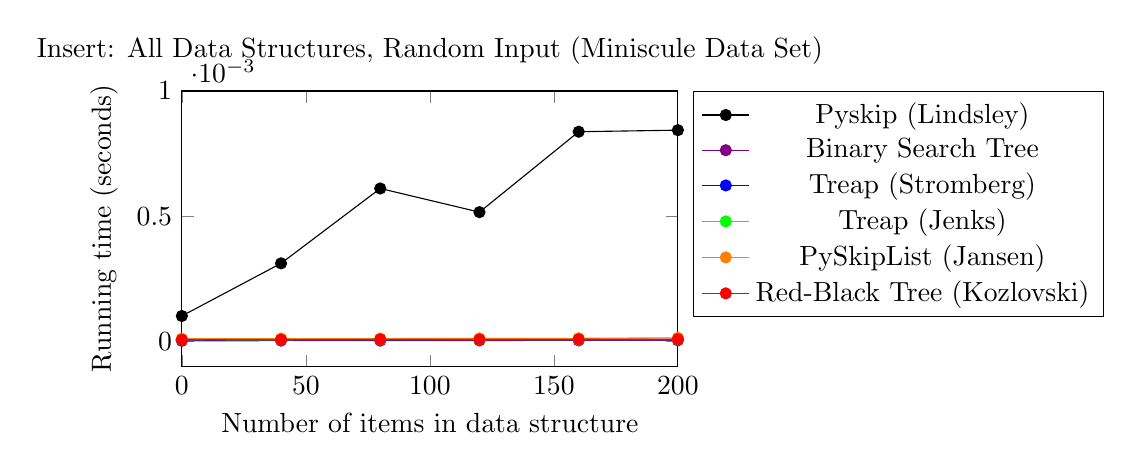
\begin{tikzpicture}
        \begin{axis}[
            title={Insert: All Data Structures, Random Input (Miniscule Data Set)},
            xmin=0, xmax=200,
            ymin=-0.0001, ymax=0.0010,
            xlabel={Number of items in data structure},
            ylabel={Running time (seconds)},
            width=0.65\textwidth,
            height=2in,
            legend pos=outer north east,
        ]
		% Pyskip
		\addplot[
		    color=black, 
		    mark=*,
	    ]
		coordinates {
			(0, 0.00010143585341796358)
			(40, 0.000311535768335931)
			(80, 0.0006105426426629923)
			(120, 0.0005160940570576679)
			(160, 0.0008371770835686271)
			(200, 0.0008434114130393855)
		};
        % BST
		\addplot[
		    color=violet,
		    mark=*,
	    ]
		coordinates {
			(0, 2.1082273572617137e-06)
			(40, 2.8912832328160653e-06)
			(80, 2.9816358338415635e-06)
			(120, 3.6743391083704157e-06)
			(160, 3.7646917093959164e-06)
			(200, 3.794809243071076e-06)
		};
		% Stromberg treap
		\addplot[
		    color=blue,
		    mark=*,
	    ]
        coordinates {
			(0, 5.1500982584523625e-06)
			(40, 6.6559749422101525e-06)
			(80, 6.3849171391350264e-06)
			(120, 6.987267812638698e-06)
			(160, 7.318560683064468e-06)
			(200, 7.288443149391921e-06)
		};
		% Jenks treap
		\addplot[
		    color=green,
		    mark=*,
	    ]
		coordinates {
			(0, 6.776445076911442e-06)
			(40, 6.625857408537605e-06)
			(80, 7.318560683064468e-06)
			(120, 6.9270327452880535e-06)
			(160, 6.776445076911442e-06)
			(200, 7.318560683064468e-06)
		};
		% PySkipList
		\addplot[
		    color=orange,
		    mark=*,
	    ]
         coordinates {
			(0, 1.0511019252634756e-05)
			(40, 1.1294075128187587e-05)
			(80, 1.108325239246033e-05)
			(120, 1.1986778402717224e-05)
			(160, 1.2287953739470447e-05)
			(200, 1.424559342835252e-05)
		};
		% Red-black tree
		\addplot[
		    color=red, 
		    mark=*,
	    ]
         coordinates {
			(0, 6.8366801442620865e-06)
			(40, 6.776445076911442e-06)
			(80, 8.101616558620073e-06)
			(120, 7.348678216742566e-06)
			(160, 8.342556828022651e-06)
			(200, 8.463026962721166e-06)
		};
        \legend{Pyskip (Lindsley), Binary Search Tree, Treap (Stromberg), Treap (Jenks), PySkipList (Jansen), Red-Black Tree (Kozlovski)}
        \end{axis}
    \end{tikzpicture}
    \caption{Average of 10 operations, benchmarked every 40, starting at 0.}
\end{figure}

Clearly Pyskip is too slow for further consideration. In fact, I began with a 105-million-element benchmark that my reference BST implementation handled in about a minute. Pyskip took so long that I eventually had to cancel the benchmark. I had to pare the initial benchmark down to below 1,000 elements to achieve a running time that would not dwarf the rest of my benchmarks combined. With Pyskip eliminated, a graph with larger (but still quite modest) data sets presents a clearer picture of the comparability of the various data structures with random inputs:

\begin{figure}[h]
    \centering
    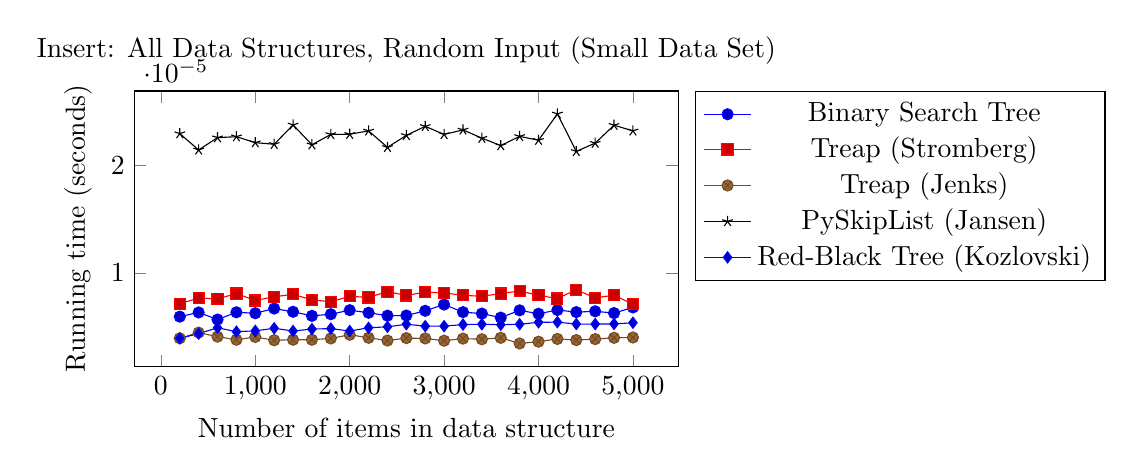
\begin{tikzpicture}
        \begin{axis}[
            xlabel={Number of items in data structure},
            ylabel={Running time (seconds)},
            title={Insert: All Data Structures, Random Input (Small Data Set)},
            width=0.7\textwidth,
            height=2in,
            legend pos=outer north east
        ]
		\addplot coordinates {
			(200, 5.933154134041274e-06)
			(400, 6.324682071845444e-06)
			(600, 5.662096330993905e-06)
			(800, 6.3397408387011465e-06)
			(1000, 6.249388237655751e-06)
			(1200, 6.686092475849392e-06)
			(1400, 6.384917139090618e-06)
			(1600, 6.00844796814215e-06)
			(1800, 6.159035636521537e-06)
			(2000, 6.535504807558823e-06)
			(2200, 6.29456453813404e-06)
			(2400, 6.023506734997852e-06)
			(2600, 6.0385655018535545e-06)
			(2800, 6.475269740136014e-06)
			(3000, 7.062561646886678e-06)
			(3200, 6.354799605468031e-06)
			(3400, 6.219270703944346e-06)
			(3600, 5.842801532995878e-06)
			(3800, 6.520446040703121e-06)
			(4000, 6.204211937088644e-06)
			(4200, 6.550563574414525e-06)
			(4400, 6.354799605468031e-06)
			(4600, 6.430093439568907e-06)
			(4800, 6.264447004422635e-06)
			(5000, 6.7915038437504904e-06)
		};
		\addplot coordinates {
			(200, 7.137855480987554e-06)
			(400, 7.664912320315409e-06)
			(600, 7.5896184861257154e-06)
			(800, 8.086557791830984e-06)
			(1000, 7.439030817746328e-06)
			(1200, 7.785382454983391e-06)
			(1400, 8.01126395764129e-06)
			(1600, 7.499265885169137e-06)
			(1800, 7.318560683078346e-06)
			(2000, 7.830558755550498e-06)
			(2200, 7.7251473876494e-06)
			(2400, 8.267262993832958e-06)
			(2600, 7.905852589740191e-06)
			(2800, 8.222086693265851e-06)
			(3000, 8.146792859164976e-06)
			(3200, 7.920911356507076e-06)
			(3400, 7.830558755550498e-06)
			(3600, 8.086557791742166e-06)
			(3800, 8.327498061166948e-06)
			(4000, 7.920911356595894e-06)
			(4200, 7.61973601983712e-06)
			(4400, 8.43290942897923e-06)
			(4600, 7.695029853937996e-06)
			(4800, 7.920911356595894e-06)
			(5000, 7.092679180509265e-06)
		};
		\addplot coordinates {
			(200, 3.915279377775249e-06)
			(400, 4.4423362171031044e-06)
			(600, 4.0658670461546365e-06)
			(800, 3.7797504762515643e-06)
			(1000, 4.035749512443232e-06)
			(1200, 3.7345741756844575e-06)
			(1400, 3.7797504761627465e-06)
			(1600, 3.7797504762515643e-06)
			(1800, 3.900220611008365e-06)
			(2000, 4.246572248156611e-06)
			(2200, 3.960455678342356e-06)
			(2400, 3.7044566420618706e-06)
			(2600, 3.930338144630951e-06)
			(2800, 3.900220610919547e-06)
			(3000, 3.6893978752061685e-06)
			(3200, 3.885161844152662e-06)
			(3400, 3.824926776729854e-06)
			(3600, 3.960455678342356e-06)
			(3800, 3.433398838925683e-06)
			(4000, 3.5990452741607727e-06)
			(4200, 3.855044310441258e-06)
			(4400, 3.7496329425401596e-06)
			(4600, 3.839985543585556e-06)
			(4800, 3.960455678253538e-06)
			(5000, 3.990573211964943e-06)
		};
		\addplot coordinates {
			(200, 2.2994736960946228e-05)
			(400, 2.147380151038547e-05)
			(600, 2.261826778999776e-05)
			(800, 2.2708620391043154e-05)
			(1000, 2.2151446018092714e-05)
			(1200, 2.2000858349713327e-05)
			(1400, 2.3807910370177156e-05)
			(1600, 2.195568204914622e-05)
			(1800, 2.2919443126845353e-05)
			(2000, 2.2934501893612236e-05)
			(2200, 2.3250735997226712e-05)
			(2400, 2.1714741779810254e-05)
			(2600, 2.2829090525799955e-05)
			(2800, 2.367238146865347e-05)
			(3000, 2.2919443126845353e-05)
			(3200, 2.334108859827211e-05)
			(3400, 2.257309148951947e-05)
			(3600, 2.1880388215045343e-05)
			(3800, 2.273873792475456e-05)
			(4000, 2.2377327520661795e-05)
			(4200, 2.483190651512146e-05)
			(4400, 2.1338272608861786e-05)
			(4600, 2.2106269717614425e-05)
			(4800, 2.3777792836554566e-05)
			(5000, 2.3250735997226712e-05)
		};
		\addplot coordinates {
			(200, 3.915279377775249e-06)
			(400, 4.351983616057708e-06)
			(600, 4.894099222241266e-06)
			(800, 4.5326888180596825e-06)
			(1000, 4.607982652338194e-06)
			(1200, 4.848922921762977e-06)
			(1400, 4.592923885482492e-06)
			(1600, 4.773629087484465e-06)
			(1800, 4.8188053880515724e-06)
			(2000, 4.592923885393674e-06)
			(2200, 4.894099222241266e-06)
			(2400, 4.984451823286662e-06)
			(2600, 5.225392092622627e-06)
			(2800, 5.044686890620653e-06)
			(3000, 5.044686890620653e-06)
			(3200, 5.1952745590000404e-06)
			(3400, 5.225392092622627e-06)
			(3600, 5.180215792144338e-06)
			(3800, 5.225392092711445e-06)
			(4000, 5.406097294713419e-06)
			(4200, 5.421156061480304e-06)
			(4400, 5.2404508594783294e-06)
			(4600, 5.2404508594783294e-06)
			(4800, 5.2555096263340316e-06)
			(5000, 5.360920994146312e-06)
		};
        \legend{Binary Search Tree, Treap (Stromberg), Treap (Jenks), PySkipList (Jansen), Red-Black Tree (Kozlovski)}
        \end{axis}
    \end{tikzpicture}
    \caption{Average of 20 operations, benchmarked every 200, starting at 200.}
\end{figure}

Based on these benchmark results, the only remaining skiplist implementation is again the clear outlier, but in this case, the difference is much less pronounced. Compared to the binary search tree reference implementation, PySkipList benchmarks on insertion at only about 2.5 times slower, and this, of course, is under ideal conditions for a binary search tree.

Comparing the Stromberg and Jenks treaps, the latter appears to be two or three times faster in this particular benchmark. Interestingly, both are comparable or superior to the binary search tree, and the Jenks treap is faster than both the binary search tree and the Kozlovski red-black tree! Because the treaps provide such interesting counterpoints, both to one another and to the deterministic data structures used here, I will keep both. Thus, the data structures are finalized.

\section{Choosing Inputs \& Benchmarks}
The remainder of this paper examines the above implementations' performance on the insert, search, and delete operations with large data sets ($10^6$ or larger). The two essential cases are randomized input and ordered input (the binary search tree's worst-case input). Beyond these, I will add as many more novel configurations as space allows.

The SIDGraphSet and SIDBenchmark classes in sidgraphset.py perform the first two benchmark sets\todo{update this}. Their sequence, in short, is to perform insertions up to each data point, benchmark searches on selected elements that have already been inserted, benchmark insertions, and repeat. Once all insertions are complete, the sequence continues with deletions: SIDBenchmark will delete elements until it reaches the last graph point plus the sample size, benchmark deletions to the graph plot point, and continue in this way until it benchmarks the first plot point. \todo{Update this to reflect any additional benchmarks.}

\section{Benchmarks: Randomized Inputs}
Random inputs are, of course, the best-case scenario for binary search tree insertions. The other data structures should perform well on randomized inputs, too. As a result, this benchmark serves as a useful baseline for later comparisons. The average-case asymptotic performance for all four data structures is $O(\log n)$, and I expect this performance from all five implementations with this input set.

\begin{figure}[h]
    \centering
    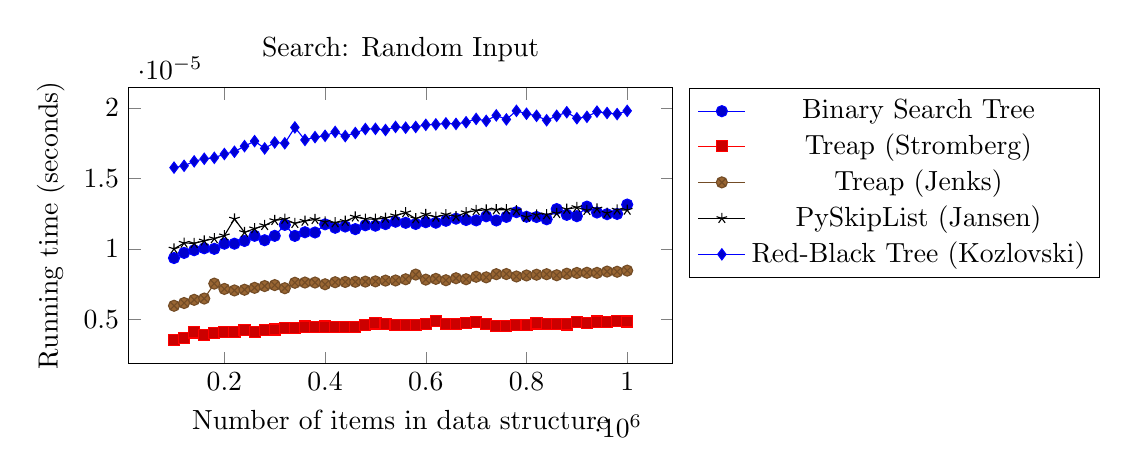
\begin{tikzpicture}
        \begin{axis}[
            xlabel={Number of items in data structure},
            ylabel={Running time (seconds)},
            title={Search: Random Input},
            width=0.7\textwidth,
            height=2in,
            legend pos=outer north east
        ]
		\addplot coordinates {
			(100000, 9.348482452771942e-06)
			(120000, 9.712001084231203e-06)
			(140000, 9.903548598405254e-06)
			(160000, 1.0040884551964058e-05)
			(180000, 9.999322355492279e-06)
			(200000, 1.0364045688298518e-05)
			(220000, 1.0365852740319204e-05)
			(240000, 1.056041200786062e-05)
			(260000, 1.0923629463983175e-05)
			(280000, 1.061070828909827e-05)
			(300000, 1.0922424762636051e-05)
			(320000, 1.1699758306792152e-05)
			(340000, 1.0920015359942248e-05)
			(360000, 1.1177821448201452e-05)
			(380000, 1.1161859155353503e-05)
			(400000, 1.1739513451243244e-05)
			(420000, 1.149556142847441e-05)
			(440000, 1.1583203451469792e-05)
			(460000, 1.1399486496050493e-05)
			(480000, 1.167235135114808e-05)
			(500000, 1.1643137343482656e-05)
			(520000, 1.1755776919427418e-05)
			(540000, 1.1924736283345893e-05)
			(560000, 1.1845527169780823e-05)
			(580000, 1.1765715705540636e-05)
			(600000, 1.1890101119619524e-05)
			(620000, 1.1854261254545584e-05)
			(640000, 1.198979015608348e-05)
			(660000, 1.2140980175133542e-05)
			(680000, 1.2046109944057193e-05)
			(700000, 1.2019004163748903e-05)
			(720000, 1.230753013635688e-05)
			(740000, 1.2013583007687955e-05)
			(760000, 1.2265967939883993e-05)
			(780000, 1.2603585492383828e-05)
			(800000, 1.2275304375325646e-05)
			(820000, 1.226084795916016e-05)
			(840000, 1.2097912101978636e-05)
			(860000, 1.2821034085519044e-05)
			(880000, 1.2410532101524653e-05)
			(900000, 1.2317167747132985e-05)
			(920000, 1.2995113430161353e-05)
			(940000, 1.2576178536738426e-05)
			(960000, 1.2460828382764078e-05)
			(980000, 1.2476790675611581e-05)
			(1000000, 1.3140581117811579e-05)
		};
		\addplot coordinates {
			(100000, 3.506885621135325e-06)
			(120000, 3.692108453240195e-06)
			(140000, 4.071890552882706e-06)
			(160000, 3.908352345028731e-06)
			(180000, 4.058036487393224e-06)
			(200000, 4.092671651118707e-06)
			(220000, 4.085443443038628e-06)
			(240000, 4.2294052540015055e-06)
			(260000, 4.1044174892519434e-06)
			(280000, 4.234826410066006e-06)
			(300000, 4.278496833894252e-06)
			(320000, 4.394449338544604e-06)
			(340000, 4.414326910769262e-06)
			(360000, 4.490524270970297e-06)
			(380000, 4.433602132323245e-06)
			(400000, 4.489319569621841e-06)
			(420000, 4.485705465580025e-06)
			(440000, 4.475164328795245e-06)
			(460000, 4.474863153458131e-06)
			(480000, 4.600453268881921e-06)
			(500000, 4.708274039437299e-06)
			(520000, 4.6896011685610975e-06)
			(540000, 4.612500282352272e-06)
			(560000, 4.603163846908842e-06)
			(580000, 4.598345041529228e-06)
			(600000, 4.650147199448895e-06)
			(620000, 4.910061515062125e-06)
			(640000, 4.693215272602913e-06)
			(660000, 4.664603615609053e-06)
			(680000, 4.745318605856142e-06)
			(700000, 4.807963075904809e-06)
			(720000, 4.6525566021387025e-06)
			(740000, 4.520039453971947e-06)
			(760000, 4.521545330653964e-06)
			(780000, 4.618222613750334e-06)
			(800000, 4.57786511862679e-06)
			(820000, 4.707972864096632e-06)
			(840000, 4.652857777472264e-06)
			(860000, 4.6844811878372635e-06)
			(880000, 4.635991958615193e-06)
			(900000, 4.8386829602549145e-06)
			(920000, 4.7254410336350365e-06)
			(940000, 4.841694713626054e-06)
			(960000, 4.8185042126931425e-06)
			(980000, 4.8537417270893e-06)
			(1000000, 4.846513519005669e-06)
		};
		\addplot coordinates {
			(100000, 5.962368141673835e-06)
			(120000, 6.157830935222819e-06)
			(140000, 6.383712437788347e-06)
			(160000, 6.475570915497997e-06)
			(180000, 7.533298698170654e-06)
			(200000, 7.1580342285813e-06)
			(220000, 7.049912282681703e-06)
			(240000, 7.099907388585791e-06)
			(260000, 7.234532764115898e-06)
			(280000, 7.3604240548732496e-06)
			(300000, 7.429393206990653e-06)
			(320000, 7.207728159137616e-06)
			(340000, 7.59383494085597e-06)
			(360000, 7.609797233698146e-06)
			(380000, 7.6113031103872685e-06)
			(400000, 7.488423572993952e-06)
			(420000, 7.632084208623268e-06)
			(440000, 7.652564131525707e-06)
			(460000, 7.664008794321831e-06)
			(480000, 7.676055807785075e-06)
			(500000, 7.693222801982813e-06)
			(520000, 7.746832011925164e-06)
			(540000, 7.757373148713497e-06)
			(560000, 7.841401067672393e-06)
			(580000, 8.17691039281243e-06)
			(600000, 7.817005865391025e-06)
			(620000, 7.870012724659148e-06)
			(640000, 7.773034266229218e-06)
			(660000, 7.916092551184307e-06)
			(680000, 7.844713996377096e-06)
			(700000, 8.019094516356517e-06)
			(720000, 7.978737021232973e-06)
			(740000, 8.202510296428045e-06)
			(760000, 8.213051433216378e-06)
			(780000, 8.039875614585413e-06)
			(800000, 8.11245887074108e-06)
			(820000, 8.166068080683431e-06)
			(840000, 8.201004419746028e-06)
			(860000, 8.127818812923238e-06)
			(880000, 8.238048986171976e-06)
			(900000, 8.291357020780765e-06)
			(920000, 8.303404034236906e-06)
			(940000, 8.295874650812607e-06)
			(960000, 8.388937829877818e-06)
			(980000, 8.374481413710555e-06)
			(1000000, 8.456099929972539e-06)
		};
		\addplot coordinates {
			(100000, 9.996611777467024e-06)
			(120000, 1.0412233742172817e-05)
			(140000, 1.0390549117929027e-05)
			(160000, 1.05670378652718e-05)
			(180000, 1.0729672547114432e-05)
			(200000, 1.093477295144396e-05)
			(220000, 1.2122006128919338e-05)
			(240000, 1.1169388538775138e-05)
			(260000, 1.143291695842663e-05)
			(280000, 1.166211138969686e-05)
			(300000, 1.2018100637746443e-05)
			(320000, 1.2103634433373145e-05)
			(340000, 1.1808783778690212e-05)
			(360000, 1.1971719635880618e-05)
			(380000, 1.2087370965190303e-05)
			(400000, 1.1907268113816372e-05)
			(420000, 1.1854261254541144e-05)
			(440000, 1.1958769096409583e-05)
			(460000, 1.226657029056355e-05)
			(480000, 1.211266969347946e-05)
			(500000, 1.2098815627993532e-05)
			(520000, 1.2180132968921954e-05)
			(540000, 1.2358729943599655e-05)
			(560000, 1.2564733873944079e-05)
			(580000, 1.2140678999799092e-05)
			(600000, 1.2439746109194517e-05)
			(620000, 1.2255727978427445e-05)
			(640000, 1.2433421427118674e-05)
			(660000, 1.2289459616155795e-05)
			(680000, 1.2574070309383956e-05)
			(700000, 1.2722248575073536e-05)
			(720000, 1.2755679037439905e-05)
			(740000, 1.277254485630408e-05)
			(760000, 1.277646013568301e-05)
			(780000, 1.2714719191649238e-05)
			(800000, 1.2255426803093883e-05)
			(820000, 1.2411435627541324e-05)
			(840000, 1.2423181465678112e-05)
			(860000, 1.251564229406199e-05)
			(880000, 1.2811095299412045e-05)
			(900000, 1.2941504220222555e-05)
			(920000, 1.2730380309164957e-05)
			(940000, 1.2839405781051027e-05)
			(960000, 1.2536122216957324e-05)
			(980000, 1.2758088440136816e-05)
			(1000000, 1.2750257881378957e-05)
		};
		\addplot coordinates {
			(100000, 1.5759903021518086e-05)
			(120000, 1.5891817819039033e-05)
			(140000, 1.6205943695268842e-05)
			(160000, 1.6391768878065704e-05)
			(180000, 1.6457726276797758e-05)
			(200000, 1.6726374677176636e-05)
			(220000, 1.688720230700369e-05)
			(240000, 1.7285958452845307e-05)
			(260000, 1.7643152402229136e-05)
			(280000, 1.7123624946350446e-05)
			(300000, 1.754587276846564e-05)
			(320000, 1.7487444753129467e-05)
			(340000, 1.8613539337252406e-05)
			(360000, 1.7723867392504644e-05)
			(380000, 1.7923245465425453e-05)
			(400000, 1.8018416871854015e-05)
			(420000, 1.8293389954294525e-05)
			(440000, 1.7998840474973577e-05)
			(460000, 1.8215686717411472e-05)
			(480000, 1.849999623530607e-05)
			(500000, 1.8514452651487544e-05)
			(520000, 1.843042473251444e-05)
			(540000, 1.8648475676315003e-05)
			(560000, 1.8593059414371284e-05)
			(580000, 1.8646969799647195e-05)
			(600000, 1.879575041598969e-05)
			(620000, 1.882827735235537e-05)
			(640000, 1.8899957082510355e-05)
			(660000, 1.8861105464083038e-05)
			(680000, 1.8979166196089635e-05)
			(700000, 1.9215890010769952e-05)
			(720000, 1.90791564078836e-05)
			(740000, 1.9467973767632428e-05)
			(760000, 1.918125484704092e-05)
			(780000, 1.9789327851952976e-05)
			(800000, 1.958061334357808e-05)
			(820000, 1.9435446831238323e-05)
			(840000, 1.912222448103762e-05)
			(860000, 1.94348444805712e-05)
			(880000, 1.968963881546415e-05)
			(900000, 1.9263475713955812e-05)
			(920000, 1.9363767101111762e-05)
			(940000, 1.9732405713284606e-05)
			(960000, 1.963452372885399e-05)
			(980000, 1.9559832245334975e-05)
			(1000000, 1.978782197525675e-05)
		};
        \legend{Binary Search Tree, Treap (Stromberg), Treap (Jenks), PySkipList (Jansen), Red-Black Tree (Kozlovski)}
        \end{axis}
    \end{tikzpicture}
    \caption{Average of 1000 operations, benchmarked every 20000, starting at 100000.}
\end{figure}

Search is perhaps the most interesting graph, because, surprisingly, the graphs of the five plots all curve to plausibly match the graph of $c \cdot \log n$ for various constant multiples $c$. Clearly, all five do in fact work in logarithmic time! (Author's note: very cool!) Both treaps are the clear winners for search. PySkipList, the slowest implementation in the small data set benchmark above, is neck-and-neck with the binary search tree. Finally, the red-black tree, the second-fastest on insertion in the small data set benchmark, is the standout slowest here.

\begin{figure}[ht]
    \centering
    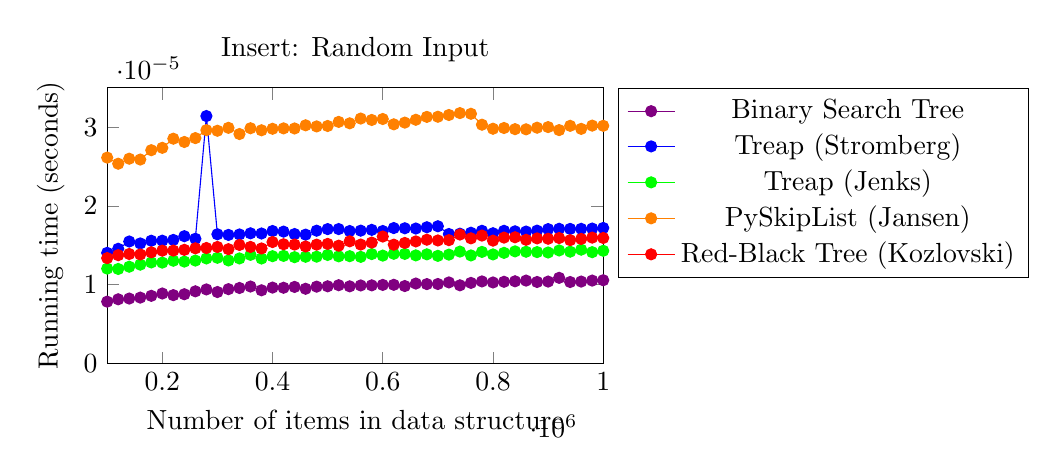
\begin{tikzpicture}
        \begin{axis}[
            title={Insert: Random Input},
            xmin=100000, xmax=1000000,
            ymin=0, ymax=0.000035,
            xlabel={Number of items in data structure},
            ylabel={Running time (seconds)},
            width=0.65\textwidth,
            height=2in,
            legend pos=outer north east,
        ]
        % BST
		\addplot[
		    color=violet,
		    mark=*,
	    ]
	    coordinates {
			(100000, 7.8380881389623e-06)
			(120000, 8.138058774366962e-06)
			(140000, 8.232025479433469e-06)
			(160000, 8.352495614134203e-06)
			(180000, 8.577473590687613e-06)
			(200000, 8.872625420704328e-06)
			(220000, 8.664513263008989e-06)
			(240000, 8.77986341698489e-06)
			(260000, 9.150911431862863e-06)
			(280000, 9.39155052592744e-06)
			(300000, 9.062365882857915e-06)
			(320000, 9.42648686499048e-06)
			(340000, 9.574966306009181e-06)
			(360000, 9.759586787438046e-06)
			(380000, 9.281621528013151e-06)
			(400000, 9.62435906123682e-06)
			(420000, 9.6047826643475e-06)
			(440000, 9.709892856874625e-06)
			(460000, 9.47557844488145e-06)
			(480000, 9.744829195937221e-06)
			(500000, 9.790005496450149e-06)
			(520000, 9.928847326691859e-06)
			(540000, 9.785186691061653e-06)
			(560000, 9.89571803965017e-06)
			(580000, 9.909270929803426e-06)
			(600000, 9.964687191765797e-06)
			(620000, 9.978541257257057e-06)
			(640000, 9.820725380798478e-06)
			(660000, 1.013846536107188e-05)
			(680000, 1.006919503361825e-05)
			(700000, 1.0080639696415261e-05)
			(720000, 1.028122247069252e-05)
			(740000, 9.915896787211054e-06)
			(760000, 1.022128857867699e-05)
			(780000, 1.0406511410780084e-05)
			(800000, 1.0275801314630683e-05)
			(820000, 1.0359226882910022e-05)
			(840000, 1.0425184281659838e-05)
			(860000, 1.051282630465522e-05)
			(880000, 1.0337241083327343e-05)
			(900000, 1.0390549117932579e-05)
			(920000, 1.0863695571970311e-05)
			(940000, 1.0332422277938847e-05)
			(960000, 1.0390247942595465e-05)
			(980000, 1.0515235707346804e-05)
			(1000000, 1.0559508481851055e-05)
		};
		% Stromberg treap
		\addplot[
		    color=blue,
		    mark=*,
	    ]
		coordinates {
			(100000, 1.4039589498015203e-05)
			(120000, 1.4554298148524935e-05)
			(140000, 1.5481918185720645e-05)
			(160000, 1.5235255584919117e-05)
			(180000, 1.557678841679433e-05)
			(200000, 1.55837154495444e-05)
			(220000, 1.5681898609322787e-05)
			(240000, 1.6155647414031192e-05)
			(260000, 1.5826763946300558e-05)
			(280000, 3.141981583128129e-05)
			(300000, 1.639959943680225e-05)
			(320000, 1.6317679745203152e-05)
			(340000, 1.637671011120645e-05)
			(360000, 1.652067192217643e-05)
			(380000, 1.6497782596584187e-05)
			(400000, 1.681220964815111e-05)
			(420000, 1.67354099372794e-05)
			(440000, 1.6428211093792554e-05)
			(460000, 1.6350809032246616e-05)
			(480000, 1.6852567143278206e-05)
			(500000, 1.705646284625928e-05)
			(520000, 1.7060980476305332e-05)
			(540000, 1.6811908472813997e-05)
			(560000, 1.6859795351358286e-05)
			(580000, 1.6958580861818008e-05)
			(600000, 1.68131131741589e-05)
			(620000, 1.718867881908892e-05)
			(640000, 1.716277774013264e-05)
			(660000, 1.7128744927077833e-05)
			(680000, 1.7291680784261132e-05)
			(700000, 1.7417270899684923e-05)
			(720000, 1.6434836951198405e-05)
			(740000, 1.6472483868298582e-05)
			(760000, 1.6592954002994986e-05)
			(780000, 1.6838110727114496e-05)
			(800000, 1.6529707182279198e-05)
			(820000, 1.6836303675091813e-05)
			(840000, 1.6773358029709585e-05)
			(860000, 1.6743541671374372e-05)
			(880000, 1.6861000052706744e-05)
			(900000, 1.7055258144914375e-05)
			(920000, 1.7094109763348797e-05)
			(940000, 1.7082062749885552e-05)
			(960000, 1.7088989782628518e-05)
			(980000, 1.7123022595683325e-05)
			(1000000, 1.7201629358574167e-05)
		};
		% Jenks treap
		\addplot[
		    color=green,
		    mark=*,
	    ]
		coordinates {
			(100000, 1.2039484086649565e-05)
			(120000, 1.1992500734116617e-05)
			(140000, 1.2276509076670549e-05)
			(160000, 1.253943514565492e-05)
			(180000, 1.2821636436193273e-05)
			(200000, 1.2798144759926799e-05)
			(220000, 1.3037579152637591e-05)
			(240000, 1.2929457206752204e-05)
			(260000, 1.3058661426214257e-05)
			(280000, 1.3328213352608031e-05)
			(300000, 1.3411337745552032e-05)
			(320000, 1.3075828420411994e-05)
			(340000, 1.3330321579964276e-05)
			(360000, 1.3785096338459368e-05)
			(380000, 1.3319780443175943e-05)
			(400000, 1.361252287050263e-05)
			(420000, 1.3652579190285507e-05)
			(440000, 1.3488438631760857e-05)
			(460000, 1.3539337263672734e-05)
			(480000, 1.3554697205847788e-05)
			(500000, 1.3771844623647667e-05)
			(520000, 1.3595054700971332e-05)
			(540000, 1.3615835799207333e-05)
			(560000, 1.3529097302217963e-05)
			(580000, 1.388327949824486e-05)
			(600000, 1.3688419055363e-05)
			(620000, 1.3920625239997263e-05)
			(640000, 1.3905867648503546e-05)
			(660000, 1.3716729537023298e-05)
			(680000, 1.3850451386531403e-05)
			(700000, 1.3657397995686438e-05)
			(720000, 1.3813105644771895e-05)
			(740000, 1.4197706549808232e-05)
			(760000, 1.3710706030295228e-05)
			(780000, 1.4157047879351126e-05)
			(800000, 1.3839307899075948e-05)
			(820000, 1.4037180095328949e-05)
			(840000, 1.4226619382128547e-05)
			(860000, 1.417963602960981e-05)
			(880000, 1.4135062079759564e-05)
			(900000, 1.4083561097180563e-05)
			(920000, 1.4344680114149355e-05)
			(940000, 1.4188370114382564e-05)
			(960000, 1.4443766799942636e-05)
			(980000, 1.4126327994986809e-05)
			(1000000, 1.4301913216314688e-05)
		};
		% PySkipList
		\addplot[
		    color=orange,
		    mark=*,
	    ]
         coordinates {
			(100000, 2.6140513353368533e-05)
			(120000, 2.5363480984538e-05)
			(140000, 2.600137034778527e-05)
			(160000, 2.5893850752552794e-05)
			(180000, 2.7081987456057278e-05)
			(200000, 2.7381355740786263e-05)
			(220000, 2.854298901462471e-05)
			(240000, 2.8125861173222688e-05)
			(260000, 2.8617680498143726e-05)
			(280000, 2.9629629629624788e-05)
			(300000, 2.9552528743408856e-05)
			(320000, 2.9923576758292826e-05)
			(340000, 2.9136003252688168e-05)
			(360000, 2.987147342503249e-05)
			(380000, 2.9612161460093488e-05)
			(400000, 2.9803106623589314e-05)
			(420000, 2.9854607606182527e-05)
			(440000, 2.9842259417378614e-05)
			(460000, 3.0244328491932037e-05)
			(480000, 3.0103679609680967e-05)
			(500000, 3.0158192345624e-05)
			(520000, 3.0678020976850465e-05)
			(540000, 3.0496713424142286e-05)
			(560000, 3.11017746756761e-05)
			(580000, 3.092167182428796e-05)
			(600000, 3.104515371236971e-05)
			(620000, 3.0368412730680915e-05)
			(640000, 3.0586162499147915e-05)
			(660000, 3.094666937724355e-05)
			(680000, 3.1314103288082154e-05)
			(700000, 3.133096910693211e-05)
			(720000, 3.155414003147427e-05)
			(740000, 3.1796586177563315e-05)
			(760000, 3.170683592720991e-05)
			(780000, 3.0321128202800196e-05)
			(800000, 2.98082266043167e-05)
			(820000, 2.9901590958715472e-05)
			(840000, 2.9756424446404138e-05)
			(860000, 2.9732631594797e-05)
			(880000, 2.9939539051156318e-05)
			(900000, 3.0018446989373615e-05)
			(920000, 2.963595431170063e-05)
			(940000, 3.0176865216503756e-05)
			(960000, 2.9790758434799614e-05)
			(980000, 3.0203970996808493e-05)
			(1000000, 3.0180780495882685e-05)
		};
		% Red-black tree
		\addplot[
		    color=red, 
		    mark=*,
	    ]
	    coordinates {
			(100000, 1.3373088477777627e-05)
			(120000, 1.3744437668009369e-05)
			(140000, 1.3894422985714527e-05)
			(160000, 1.3836597321045474e-05)
			(180000, 1.4110064526818178e-05)
			(200000, 1.4316670807829724e-05)
			(220000, 1.4324501366587583e-05)
			(240000, 1.4420576298988409e-05)
			(260000, 1.4613930865209567e-05)
			(280000, 1.4654890711000235e-05)
			(300000, 1.4788010209827007e-05)
			(320000, 1.4504303042627952e-05)
			(340000, 1.5042202194081256e-05)
			(360000, 1.4789817261885218e-05)
			(380000, 1.4598872098360971e-05)
			(400000, 1.541053963092054e-05)
			(420000, 1.513014539239066e-05)
			(440000, 1.5087980845237326e-05)
			(460000, 1.4850955855251868e-05)
			(480000, 1.5080451461813027e-05)
			(500000, 1.5176526394242274e-05)
			(520000, 1.4948837839654062e-05)
			(540000, 1.5505108686653557e-05)
			(560000, 1.509249847529759e-05)
			(580000, 1.5340666952795345e-05)
			(600000, 1.6112278165536507e-05)
			(620000, 1.5078644409811659e-05)
			(640000, 1.5295791827611538e-05)
			(660000, 1.549245932250187e-05)
			(680000, 1.5706896162271278e-05)
			(700000, 1.561232710653826e-05)
			(720000, 1.5653286952357347e-05)
			(740000, 1.6362554870397615e-05)
			(760000, 1.5882180208251385e-05)
			(780000, 1.6232447124906456e-05)
			(800000, 1.5591847183628714e-05)
			(820000, 1.5977050439346384e-05)
			(840000, 1.6017709109803492e-05)
			(860000, 1.569755972684561e-05)
			(880000, 1.587555435085619e-05)
			(900000, 1.5830378050367245e-05)
			(920000, 1.5918923599372193e-05)
			(940000, 1.5653588127662488e-05)
			(960000, 1.5809898127429277e-05)
			(980000, 1.597223163395256e-05)
			(1000000, 1.593036826213279e-05)
		};
        \legend{Binary Search Tree, Treap (Stromberg), Treap (Jenks), PySkipList (Jansen), Red-Black Tree (Kozlovski)}
        \end{axis}
    \end{tikzpicture}
    \caption{Average of 1000 operations, benchmarked every 20000, starting at 100000.}
    \label{fig:random_insert}
\end{figure}

Next up is insertion. Here, the logarithmic graph is faintly visible at best. The most telling is perhaps the binary search tree, whose running time approximately doubles from $10^5$ elements to $10^6$ elements, in keeping with a logarithmic rate of growth.  In comparison to the small data set insertion benchmark, almost everything is the same: the treaps and red-black tree are all tightly grouped, and PySkipList takes about twice as long as the rest. However, in this best-case input for the binary search tree, it does indeed pull ahead of the pack.

\begin{figure}[h]
    \centering
    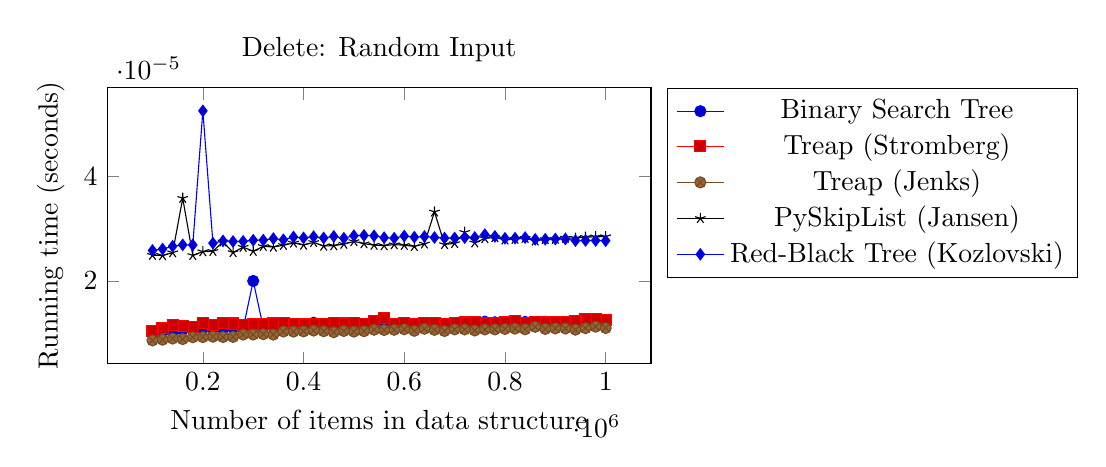
\begin{tikzpicture}
        \begin{axis}[
            xlabel={Number of items in data structure},
            ylabel={Running time (seconds)},
            title={Delete: Random Input},
            width=0.7\textwidth,
            height=2in,
            legend pos=outer north east
        ]
		\addplot coordinates {
			(1000000, 1.2300301928275913e-05)
			(980000, 1.2457515454059375e-05)
			(960000, 1.1958166745726472e-05)
			(940000, 1.2082552159803583e-05)
			(920000, 1.21256202329576e-05)
			(900000, 1.1965997304480779e-05)
			(880000, 1.2193987034400778e-05)
			(860000, 1.1927446861376367e-05)
			(840000, 1.2181638845595088e-05)
			(820000, 1.1870825898068205e-05)
			(800000, 1.2046712294731422e-05)
			(780000, 1.2106345011407172e-05)
			(760000, 1.2221092814709068e-05)
			(740000, 1.1908773990498388e-05)
			(720000, 1.2090985069233895e-05)
			(700000, 1.1793423836522265e-05)
			(680000, 1.1666629019750019e-05)
			(660000, 1.1665725493740452e-05)
			(640000, 1.180667555133752e-05)
			(620000, 1.1618742141209282e-05)
			(600000, 1.1594648114265028e-05)
			(580000, 1.158109522411266e-05)
			(560000, 1.1640125590112405e-05)
			(540000, 1.1984369000021644e-05)
			(520000, 1.1635909135399914e-05)
			(500000, 1.1477792083606885e-05)
			(480000, 1.1401293548068736e-05)
			(460000, 1.1464239193450964e-05)
			(440000, 1.1498573181842886e-05)
			(420000, 1.201358300768618e-05)
			(400000, 1.1264559945185938e-05)
			(380000, 1.1401293548072289e-05)
			(360000, 1.1195590793068533e-05)
			(340000, 1.1337745552015832e-05)
			(320000, 1.1104635841370225e-05)
			(300000, 2.00251481406184e-05)
			(280000, 1.0921220061291591e-05)
			(260000, 1.103145023454033e-05)
			(240000, 1.0792015841822433e-05)
			(220000, 1.0889596650933697e-05)
			(200000, 1.0902547190411837e-05)
			(180000, 1.0643536400806396e-05)
			(160000, 1.0664317499042397e-05)
			(140000, 1.0217975649972288e-05)
			(120000, 1.0283029522714315e-05)
			(100000, 9.972818925859883e-06)
		};
		\addplot coordinates {
			(1000000, 1.2546663353738552e-05)
			(980000, 1.2764111946871993e-05)
			(960000, 1.2721345049051535e-05)
			(940000, 1.2289158440815129e-05)
			(920000, 1.2191276456370304e-05)
			(900000, 1.2127728460313847e-05)
			(880000, 1.204912169743011e-05)
			(860000, 1.2097008575970847e-05)
			(840000, 1.2014787709034636e-05)
			(820000, 1.2422880290337446e-05)
			(800000, 1.2111766167471672e-05)
			(780000, 1.199280190945018e-05)
			(760000, 1.1906364587801477e-05)
			(740000, 1.2110862641463883e-05)
			(720000, 1.2046712294726092e-05)
			(700000, 1.1980453720639161e-05)
			(680000, 1.1834684857660705e-05)
			(660000, 1.201267948167839e-05)
			(640000, 1.202141356644404e-05)
			(620000, 1.1734393470518967e-05)
			(600000, 1.1941903277538302e-05)
			(580000, 1.1793725011862932e-05)
			(560000, 1.2936685414835836e-05)
			(540000, 1.2329214760605113e-05)
			(520000, 1.1739814626579914e-05)
			(500000, 1.2034665281262846e-05)
			(480000, 1.1856068306563827e-05)
			(460000, 1.1985573701366547e-05)
			(440000, 1.1703673586168862e-05)
			(420000, 1.1708492391562686e-05)
			(400000, 1.1666026669075792e-05)
			(380000, 1.1798543817242546e-05)
			(360000, 1.1964190252463424e-05)
			(340000, 1.1855164780556037e-05)
			(320000, 1.1697348904093019e-05)
			(300000, 1.1740416977254142e-05)
			(280000, 1.1616633913853035e-05)
			(260000, 1.186570591734437e-05)
			(240000, 1.1888896418277283e-05)
			(220000, 1.1656389058302352e-05)
			(200000, 1.193768682282581e-05)
			(180000, 1.1158245051312576e-05)
			(160000, 1.1464540368791631e-05)
			(140000, 1.152447426080272e-05)
			(120000, 1.0933267074754837e-05)
			(100000, 1.048511817366915e-05)
		};
		\addplot coordinates {
			(1000000, 1.1007356207613839e-05)
			(980000, 1.1271486977932454e-05)
			(960000, 1.0973925745219048e-05)
			(940000, 1.069323033136982e-05)
			(920000, 1.0922424762640049e-05)
			(900000, 1.0929050620035241e-05)
			(880000, 1.083568626565068e-05)
			(860000, 1.1239261216886121e-05)
			(840000, 1.0764608886177029e-05)
			(820000, 1.0891102527608609e-05)
			(800000, 1.0829361583574836e-05)
			(780000, 1.0742321911266117e-05)
			(760000, 1.073479252784182e-05)
			(740000, 1.0538727383618606e-05)
			(720000, 1.0735696053856713e-05)
			(700000, 1.0745634839963714e-05)
			(680000, 1.0434219541764378e-05)
			(660000, 1.0656486940277431e-05)
			(640000, 1.0867008500682118e-05)
			(620000, 1.047608291356994e-05)
			(600000, 1.0775451198298924e-05)
			(580000, 1.0668533953747784e-05)
			(560000, 1.062998351065403e-05)
			(540000, 1.0676665687853415e-05)
			(520000, 1.0403198482080711e-05)
			(500000, 1.0320977615137395e-05)
			(480000, 1.044054422382601e-05)
			(460000, 1.0208036863872394e-05)
			(440000, 1.0398379676686886e-05)
			(420000, 1.0518247460723274e-05)
			(400000, 1.0364949214320519e-05)
			(380000, 1.0322784667167185e-05)
			(360000, 1.0336939907986676e-05)
			(340000, 9.744829195938109e-06)
			(320000, 9.827351238214987e-06)
			(300000, 9.763200891470091e-06)
			(280000, 9.751455053347512e-06)
			(260000, 9.310835535671913e-06)
			(240000, 9.285235632049193e-06)
			(220000, 9.346675400749405e-06)
			(200000, 9.273790969245965e-06)
			(180000, 9.241866383561615e-06)
			(160000, 8.89310534361698e-06)
			(140000, 8.987674399349998e-06)
			(120000, 8.772032858232137e-06)
			(100000, 8.634998080012224e-06)
		};
		\addplot coordinates {
			(1000000, 2.8524316143744955e-05)
			(980000, 2.8486066875984762e-05)
			(960000, 2.8402942483040762e-05)
			(940000, 2.8236994872486322e-05)
			(920000, 2.824060897653169e-05)
			(900000, 2.8022256857383355e-05)
			(880000, 2.798250171292693e-05)
			(860000, 2.769487926633474e-05)
			(840000, 2.8212599670212057e-05)
			(820000, 2.8027979188777863e-05)
			(800000, 2.7883716202481423e-05)
			(780000, 2.8350839149780426e-05)
			(760000, 2.8164712791664214e-05)
			(740000, 2.7331059459541508e-05)
			(720000, 2.9360378878578786e-05)
			(700000, 2.721119167551933e-05)
			(680000, 2.7018138284660152e-05)
			(660000, 3.326511711955504e-05)
			(640000, 2.7125657879864208e-05)
			(620000, 2.664347616574503e-05)
			(600000, 2.6866647090272977e-05)
			(580000, 2.699133367967477e-05)
			(560000, 2.6790449730071942e-05)
			(540000, 2.6887729363849643e-05)
			(520000, 2.7164810673667717e-05)
			(500000, 2.7594587879207212e-05)
			(480000, 2.7077771001330574e-05)
			(460000, 2.6794666184798645e-05)
			(440000, 2.6712144142521765e-05)
			(420000, 2.741870148255998e-05)
			(400000, 2.6903691656713135e-05)
			(380000, 2.7306965432615016e-05)
			(360000, 2.6853094200106396e-05)
			(340000, 2.6524511907723536e-05)
			(320000, 2.6656426705216063e-05)
			(300000, 2.571916905725402e-05)
			(280000, 2.6496803776751678e-05)
			(260000, 2.5480337015210352e-05)
			(240000, 2.7526221077749823e-05)
			(220000, 2.571314555049753e-05)
			(200000, 2.5638755242340493e-05)
			(180000, 2.4918042661482787e-05)
			(160000, 3.587480141251831e-05)
			(140000, 2.5439075994057704e-05)
			(120000, 2.4890033355177365e-05)
			(100000, 2.4956291929271402e-05)
		};
		\addplot coordinates {
			(1000000, 2.7731622657427123e-05)
			(980000, 2.7773184853884915e-05)
			(960000, 2.7774991905914703e-05)
			(940000, 2.7746681424247298e-05)
			(920000, 2.8065927281232915e-05)
			(900000, 2.8054482618415476e-05)
			(880000, 2.8013823947958372e-05)
			(860000, 2.7998464005776214e-05)
			(840000, 2.8328250999521742e-05)
			(820000, 2.821862317694013e-05)
			(800000, 2.8194529150027846e-05)
			(780000, 2.8555638378776392e-05)
			(760000, 2.8895966509281835e-05)
			(740000, 2.8349032097764848e-05)
			(720000, 2.832915452555085e-05)
			(700000, 2.8256270094033197e-05)
			(680000, 2.823488664512297e-05)
			(660000, 2.835505560449292e-05)
			(640000, 2.8538471384564446e-05)
			(620000, 2.842101300322497e-05)
			(600000, 2.8636955719690604e-05)
			(580000, 2.8222237280971285e-05)
			(560000, 2.831409575870225e-05)
			(540000, 2.8669482656084712e-05)
			(520000, 2.8749896470969817e-05)
			(500000, 2.8695986085693903e-05)
			(480000, 2.821711730027232e-05)
			(460000, 2.8558650132140428e-05)
			(440000, 2.8263498302123936e-05)
			(420000, 2.850624562353232e-05)
			(400000, 2.8274039438912267e-05)
			(380000, 2.8439685874133147e-05)
			(360000, 2.7911123158133934e-05)
			(340000, 2.81382093620266e-05)
			(320000, 2.783944342797895e-05)
			(300000, 2.7825288187131035e-05)
			(280000, 2.761024899672293e-05)
			(260000, 2.7576517358994578e-05)
			(240000, 2.769758984436521e-05)
			(220000, 2.7259078554038753e-05)
			(200000, 5.2615632505848e-05)
			(180000, 2.6921762176897345e-05)
			(160000, 2.693049626165589e-05)
			(140000, 2.666997959536843e-05)
			(120000, 2.613960982736785e-05)
			(100000, 2.5870057900959863e-05)
		};
        \legend{Binary Search Tree, Treap (Stromberg), Treap (Jenks), PySkipList (Jansen), Red-Black Tree (Kozlovski)}
        \end{axis}
    \end{tikzpicture}
    \caption{Average of 1000 operations, benchmarked every 20000, starting at 100000.}
\end{figure}

Finally, delete performance is almost entirely flat across all five graphs. It is stratified into two groups, but on closer inspection, these are easily explained. Binary search trees and treaps both enjoy relatively simple insertions and deletions, whereas red-black trees and skip lists \todo{confirm this} may require much more work for both.

\section{Benchmarks: Ordered Inputs}

The worst-case scenarios for binary search trees are inserting ordered data, deleting the farthest leaf, and searching for the lowest data in the tree. In any of these cases, the worst-case performance is $O(n)$. Since treaps, skiplists, and red-black trees all claim to run in $O(\log n)$ expected time in these scenarioes, these worst-case inputs are the next logical benchmark. To briefly illustrate the performance difference between the binary search tree and all the other data structures, see the mini-graphs with the binary search tree clearly dwarfing the other data structures and performing in linear time. This is expected and needs no further discussion. (Note that for these graphs, the benchmark parameters were adjusted: the normal 180 million overall searches, insertions, and deletions would take unreasonably long and provide no noticeable benefit in terms of graph quality.)

The more interesting graphs appear when the binary search tree is removed from the data set, as appears below. 

\begin{figure}[h]
    \centering
    \begin{figure}[h]
    \centering
    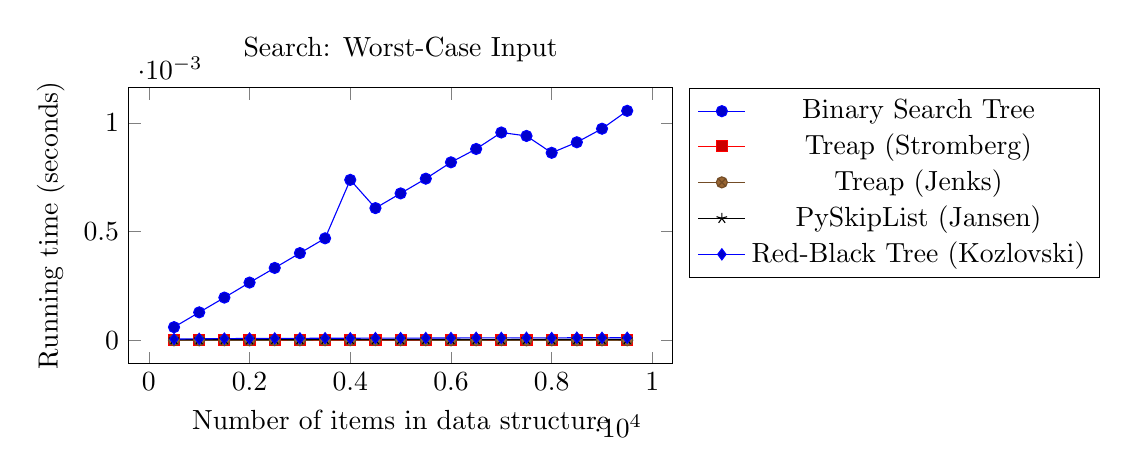
\begin{tikzpicture}
        \begin{axis}[
            xlabel={Number of items in data structure},
            ylabel={Running time (seconds)},
            title={Search: Worst-Case Input},
            width=0.7\textwidth,
            height=2in,
            legend pos=outer north east
        ]
		\addplot coordinates {
			(500, 6.181924962164849e-05)
			(1000, 0.00012983668767364633)
			(1500, 0.00019761017370287543)
			(2000, 0.00026660040809258157)
			(2500, 0.0003338679195560673)
			(3000, 0.00040190945163500635)
			(3500, 0.00046979136078546536)
			(4000, 0.0007382590559659064)
			(4500, 0.0006085247679067552)
			(5000, 0.000676150678020977)
			(5500, 0.0007437856233952989)
			(6000, 0.0008188204467936133)
			(6500, 0.0008801517923697232)
			(7000, 0.0009557708959213329)
			(7500, 0.0009399772612620705)
			(8000, 0.0008625029176360765)
			(8500, 0.000910904806005437)
			(9000, 0.0009731035365513918)
			(9500, 0.0010552701919239826)
		};
		\addplot coordinates {
			(500, 1.075195952200403e-06)
			(1000, 1.0842312123138243e-06)
			(1500, 1.2107248537418513e-06)
			(2000, 1.572135257834617e-06)
			(2500, 1.6594761055088724e-06)
			(3000, 1.3552890153789577e-06)
			(3500, 1.4275710961975108e-06)
			(4000, 1.4275710961975108e-06)
			(4500, 1.5480412309010206e-06)
			(5000, 1.7227229262317679e-06)
			(5500, 1.9245104018494884e-06)
			(6000, 1.716699419489487e-06)
			(6500, 1.2559011542556674e-06)
			(7000, 1.313124468236282e-06)
			(7500, 1.5932175314148367e-06)
			(8000, 1.358300768750098e-06)
			(8500, 1.3733595355880369e-06)
			(9000, 1.578158764576898e-06)
			(9500, 1.551052984272161e-06)
		};
		\addplot coordinates {
			(500, 1.6173115583484333e-06)
			(1000, 1.7468169531653643e-06)
			(1500, 1.8702988412400145e-06)
			(2000, 1.5781587645946615e-06)
			(2500, 2.0479922899241388e-06)
			(3000, 1.870298841222251e-06)
			(3500, 2.0750980702288757e-06)
			(4000, 1.933545661945146e-06)
			(4500, 2.273873792475456e-06)
			(5000, 1.948604428783085e-06)
			(5500, 2.041968783181858e-06)
			(6000, 1.6293585718152315e-06)
			(6500, 1.8401813075463736e-06)
			(7000, 2.1202743707249283e-06)
			(7500, 1.502864930404968e-06)
			(8000, 1.578158764576898e-06)
			(8500, 1.7588639666143991e-06)
			(9000, 1.7227229262140043e-06)
			(9500, 1.7377816930697065e-06)
		};
		\addplot coordinates {
			(500, 5.0025223434424504e-06)
			(1000, 4.300783808801612e-06)
			(1500, 5.035651630489468e-06)
			(2000, 4.2495840015632776e-06)
			(2500, 5.580778990008639e-06)
			(3000, 4.960357796299775e-06)
			(3500, 5.78256646562636e-06)
			(4000, 5.734378411741403e-06)
			(4500, 4.653158952798719e-06)
			(5000, 4.538712324837491e-06)
			(5500, 5.580778990008639e-06)
			(6000, 4.891087468852362e-06)
			(6500, 4.981440069879994e-06)
			(7000, 4.698335253330299e-06)
			(7500, 5.228403846011531e-06)
			(8000, 4.897110975576879e-06)
			(8500, 4.9483107828329765e-06)
			(9000, 5.656072824198332e-06)
			(9500, 5.264544886411926e-06)
		};
		\addplot coordinates {
			(500, 7.2583256157088275e-06)
			(1000, 8.243168966899361e-06)
			(1500, 9.375588233080378e-06)
			(2000, 9.66471655635459e-06)
			(2500, 1.0179726382197884e-05)
			(3000, 1.04447606785385e-05)
			(3500, 1.0986876284686531e-05)
			(4000, 1.070678322152574e-05)
			(4500, 1.1757885146774783e-05)
			(5000, 1.1547062411061404e-05)
			(5500, 1.1857273007915837e-05)
			(6000, 1.1893414048333994e-05)
			(6500, 1.2968610000534397e-05)
			(7000, 1.2366259327034611e-05)
			(7500, 1.2992704027467994e-05)
			(8000, 1.203195470322882e-05)
			(8500, 1.3525784373520367e-05)
			(9000, 1.2851151619202027e-05)
			(9500, 1.3167385722780977e-05)
		};
        \legend{Binary Search Tree, Treap (Stromberg), Treap (Jenks), PySkipList (Jansen), Red-Black Tree (Kozlovski)}
        \end{axis}
    \end{tikzpicture}
    \caption{Average of 100 operations, benchmarked every 500, starting at 500.}
\end{figure}
        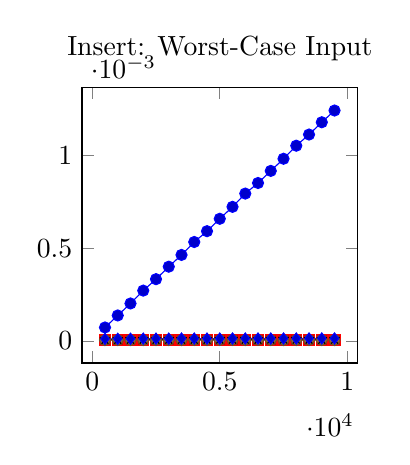
\begin{tikzpicture}
        \begin{axis}[
            title={Insert: Worst-Case Input},
            width=2in,
            height=2in,
        ]
		\addplot coordinates {
			(500, 7.212245789192323e-05)
			(1000, 0.00013702875471527625)
			(1500, 0.000201763381596681)
			(2000, 0.00027111201463712154)
			(2500, 0.0003329101819851965)
			(3000, 0.0004002047992289903)
			(3500, 0.00046372870125665377)
			(4000, 0.000533420674180991)
			(4500, 0.0005918276072372453)
			(5000, 0.0006587035907629501)
			(5500, 0.0007231912538682206)
			(6000, 0.0007947535256337846)
			(6500, 0.0008518051696746554)
			(7000, 0.0009171090179425212)
			(7500, 0.0009825514068652907)
			(8000, 0.001053056553198859)
			(8500, 0.001113264514768879)
			(9000, 0.0011795562181412932)
			(9500, 0.0012428813444467046)
		};
		\addplot coordinates {
			(500, 4.851934675080827e-06)
			(1000, 4.830852401482844e-06)
			(1500, 4.433300956989683e-06)
			(2000, 5.475367622160832e-06)
			(2500, 5.764495945399517e-06)
			(3000, 4.767605580795475e-06)
			(3500, 4.897110975576879e-06)
			(4000, 5.83075451952908e-06)
			(4500, 5.716307891532324e-06)
			(5000, 4.4875125175991574e-06)
			(5500, 6.101812322611977e-06)
			(6000, 5.797625232482062e-06)
			(6500, 5.866895559911711e-06)
			(7000, 5.216356832562497e-06)
			(7500, 5.0416751372495125e-06)
			(8000, 4.285725041981437e-06)
			(8500, 4.586900378740211e-06)
			(9000, 5.565720223188464e-06)
			(9500, 6.011459721548817e-06)
		};
		\addplot coordinates {
			(500, 4.231513481336435e-06)
			(1000, 4.604970898931526e-06)
			(1500, 4.189348934211523e-06)
			(2000, 4.354995369446613e-06)
			(2500, 4.629064925865123e-06)
			(3000, 4.490524270970297e-06)
			(3500, 4.586900378740211e-06)
			(4000, 4.836875908260652e-06)
			(4500, 4.731464540377317e-06)
			(5000, 4.90012272894802e-06)
			(5500, 5.104921957936881e-06)
			(6000, 4.4031834233138055e-06)
			(6500, 5.041675137213985e-06)
			(7000, 4.553771091693193e-06)
			(7500, 4.2797015352391556e-06)
			(8000, 4.61099440563828e-06)
			(8500, 4.592923885482492e-06)
			(9000, 4.351983616039945e-06)
			(9500, 4.270666275125734e-06)
		};
		\addplot coordinates {
			(500, 7.938981876804974e-06)
			(1000, 8.201004419738923e-06)
			(1500, 9.083448156417263e-06)
			(2000, 8.899731200990858e-06)
			(2500, 7.932958370062693e-06)
			(3000, 9.354505959535686e-06)
			(3500, 8.794319833143049e-06)
			(4000, 8.6708379450684e-06)
			(4500, 8.80034333988533e-06)
			(5000, 1.0029138713818498e-05)
			(5500, 9.60146973564946e-06)
			(6000, 9.294270892148404e-06)
			(6500, 8.30641578758673e-06)
			(7000, 1.0315255283757097e-05)
			(7500, 1.0294173010194641e-05)
			(8000, 9.718928116981829e-06)
			(8500, 9.459917327383493e-06)
			(9000, 8.490132743013135e-06)
			(9500, 9.047307116034632e-06)
		};
		\addplot coordinates {
			(500, 1.0550172046421835e-05)
			(1000, 1.1086264145809821e-05)
			(1500, 1.1438639289806928e-05)
			(2000, 1.1637415012089036e-05)
			(2500, 1.1851249501155791e-05)
			(3000, 1.1941602102218952e-05)
			(3500, 1.2122307304274216e-05)
			(4000, 1.213134256435211e-05)
			(4500, 1.2333130040005359e-05)
			(5000, 1.2293977246216059e-05)
			(5500, 1.2402400367435007e-05)
			(6000, 1.240842387414176e-05)
			(6500, 1.2682493430595799e-05)
			(7000, 1.2625270116650712e-05)
			(7500, 1.2673458170517903e-05)
			(8000, 1.264936414354878e-05)
			(8500, 1.3019809807808257e-05)
			(9000, 1.2998727534210275e-05)
			(9500, 1.3022821561143872e-05)
		};
        \end{axis}
    \end{tikzpicture}
    \begin{figure}[h]
    \centering
    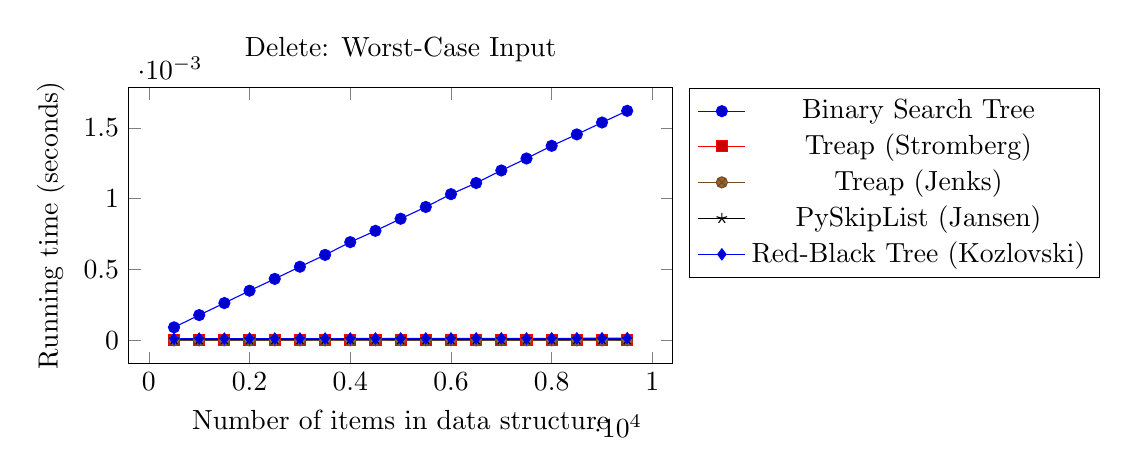
\begin{tikzpicture}
        \begin{axis}[
            xlabel={Number of items in data structure},
            ylabel={Running time (seconds)},
            title={Delete: Worst-Case Input},
            width=0.7\textwidth,
            height=2in,
            legend pos=outer north east
        ]
		\addplot coordinates {
			(9500, 0.0016196366319561762)
			(9000, 0.0015374488943100317)
			(8500, 0.0014535384337376555)
			(8000, 0.001373019207457098)
			(7500, 0.0012837146966034752)
			(7000, 0.0011992832026985311)
			(6500, 0.0011108611355816222)
			(6000, 0.0010323447252904216)
			(5500, 0.0009421125943996245)
			(5000, 0.0008589972367163056)
			(4500, 0.0007737435341419996)
			(4000, 0.0006942031277058547)
			(3500, 0.0006041757960440819)
			(3000, 0.0005206899926965036)
			(2500, 0.00043513210303210316)
			(2000, 0.0003517426757922948)
			(1500, 0.0002646548154171313)
			(1000, 0.00017986793461481908)
			(500, 9.353602433492369e-05)
		};
		\addplot coordinates {
			(9500, 3.0810236949463387e-06)
			(9000, 3.1804115560873923e-06)
			(8500, 2.906341999633355e-06)
			(8000, 2.782860111594232e-06)
			(7500, 2.267850285733175e-06)
			(7000, 3.2496818835170416e-06)
			(6500, 3.475563386103886e-06)
			(6000, 3.035847394414759e-06)
			(5500, 3.5297749467133597e-06)
			(5000, 3.0539179146416017e-06)
			(4500, 2.8430951788749325e-06)
			(4000, 3.168364542673885e-06)
			(3500, 2.8340599187970383e-06)
			(3000, 2.5961314027966864e-06)
			(2500, 1.9516161821542253e-06)
			(2000, 3.882150090745995e-06)
			(1500, 4.228501727965295e-06)
			(1000, 3.430387085572306e-06)
			(500, 2.547943348858439e-06)
		};
		\addplot coordinates {
			(9500, 2.0058277427636993e-06)
			(9000, 1.8100637738882598e-06)
			(8500, 2.1624389178498403e-06)
			(8000, 1.9305339085207154e-06)
			(7500, 2.186532944818964e-06)
			(7000, 2.538908088851599e-06)
			(6500, 2.047992289959666e-06)
			(6000, 2.28290905255335e-06)
			(5500, 2.1323213842094903e-06)
			(5000, 1.975710209052295e-06)
			(4500, 2.1293096308028226e-06)
			(4000, 2.2256857385372085e-06)
			(3500, 1.8401813075996642e-06)
			(3000, 1.8522283210131717e-06)
			(2500, 2.029921769732823e-06)
			(2000, 1.6052645449349256e-06)
			(1500, 1.8733105946466821e-06)
			(1000, 1.7528404598721181e-06)
			(500, 1.8221107873017673e-06)
		};
		\addplot coordinates {
			(9500, 7.1890552882081235e-06)
			(9000, 9.375588233098142e-06)
			(8500, 8.194980912961114e-06)
			(8000, 7.586606732772339e-06)
			(7500, 7.429995557686197e-06)
			(7000, 7.797429468539008e-06)
			(6500, 7.460113091326548e-06)
			(6000, 7.4360190644284786e-06)
			(5500, 6.984256059254789e-06)
			(5000, 7.354701723514267e-06)
			(4500, 9.14669497710463e-06)
			(4000, 9.360529466277967e-06)
			(3500, 9.547258175075513e-06)
			(3000, 7.2733843825290026e-06)
			(2500, 7.652865306866374e-06)
			(2000, 8.032346231132693e-06)
			(1500, 6.987267812590403e-06)
			(1000, 6.86378592455128e-06)
			(500, 6.586704614761629e-06)
		};
		\addplot coordinates {
			(9500, 1.7091700360651885e-05)
			(9000, 1.6308644485150127e-05)
			(8500, 1.637189130576644e-05)
			(8000, 1.5649070497616434e-05)
			(7500, 1.5736411345272927e-05)
			(7000, 1.567617627792117e-05)
			(6500, 1.5757493618835384e-05)
			(6000, 1.50105787836452e-05)
			(5500, 1.5082860864481517e-05)
			(5000, 1.4947331962957832e-05)
			(4500, 1.5022625797129763e-05)
			(4000, 1.4516651231417655e-05)
			(3500, 1.4459427917401513e-05)
			(3000, 1.4450392657394672e-05)
			(2500, 1.4417263370276601e-05)
			(2000, 1.4125123293666774e-05)
			(1500, 1.379383042326765e-05)
			(1000, 1.3634207494703787e-05)
			(500, 1.30830566284601e-05)
		};
        \legend{Binary Search Tree, Treap (Stromberg), Treap (Jenks), PySkipList (Jansen), Red-Black Tree (Kozlovski)}
        \end{axis}
    \end{tikzpicture}
    \caption{Average of 100 operations, benchmarked every 500, starting at 500.}
\end{figure}
    \caption{Average of 100 operations, benchmarked every 500, starting at 500.}
\end{figure}

\begin{figure}[h]
    \centering
    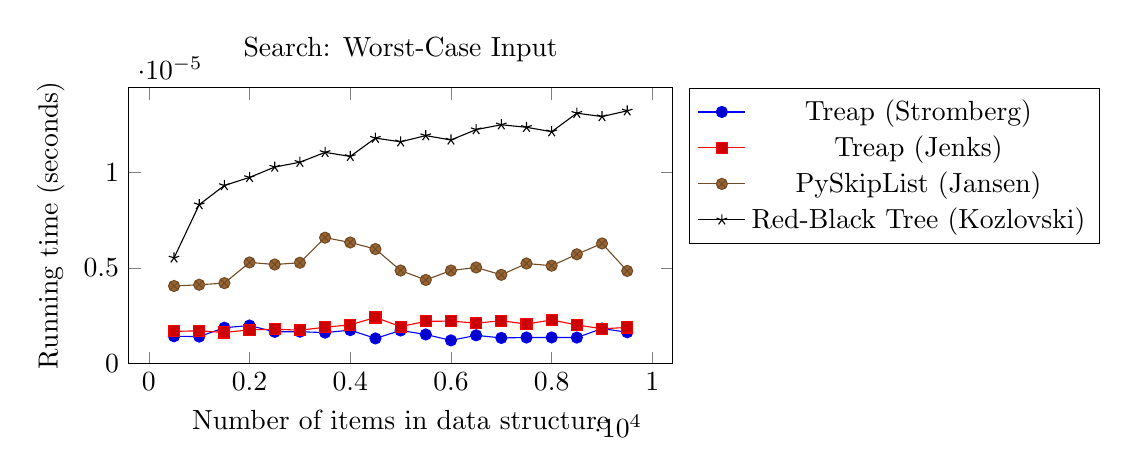
\begin{tikzpicture}
        \begin{axis}[
            xlabel={Number of items in data structure},
            ylabel={Running time (seconds)},
            title={Search: Worst-Case Input},
            width=0.7\textwidth,
            height=2in,
            legend pos=outer north east
        ]
		\addplot coordinates {
			(500, 1.4125123293950991e-06)
			(1000, 1.3944418091682564e-06)
			(1500, 1.8612635811621204e-06)
			(2000, 1.975710209052295e-06)
			(2500, 1.6444173386531703e-06)
			(3000, 1.6534525988021187e-06)
			(3500, 1.602252791528258e-06)
			(4000, 1.7347699397163296e-06)
			(4500, 1.298065701362816e-06)
			(5000, 1.716699419489487e-06)
			(5500, 1.505876683793872e-06)
			(6000, 1.1956660869572034e-06)
			(6500, 1.4607003832622923e-06)
			(7000, 1.3251714817386073e-06)
			(7500, 1.3462537553010635e-06)
			(8000, 1.3492655086366767e-06)
			(8500, 1.3432420019654502e-06)
			(9000, 1.8160872805594863e-06)
			(9500, 1.623335065090714e-06)
		};
		\addplot coordinates {
			(500, 1.6685113655512395e-06)
			(1000, 1.6986288992626442e-06)
			(1500, 1.6112880516772065e-06)
			(2000, 1.7498287065365049e-06)
			(2500, 1.7829579935124684e-06)
			(3000, 1.7317581863096621e-06)
			(3500, 1.8853576080601897e-06)
			(4000, 2.0118512495059805e-06)
			(4500, 2.4003674339212464e-06)
			(5000, 1.9184868951072076e-06)
			(5500, 2.1955682048968585e-06)
			(6000, 2.20761521838142e-06)
			(6500, 2.1022038504980856e-06)
			(7000, 2.2256857385372085e-06)
			(7500, 2.0510040432952794e-06)
			(8000, 2.270862039068788e-06)
			(8500, 2.002815989357032e-06)
			(9000, 1.807052020481592e-06)
			(9500, 1.8733105946466821e-06)
		};
		\addplot coordinates {
			(500, 4.0508082793166975e-06)
			(1000, 4.117066853410734e-06)
			(1500, 4.201395947731612e-06)
			(2000, 5.288638913327759e-06)
			(2500, 5.180215792108811e-06)
			(3000, 5.273580146578638e-06)
			(3500, 6.589716368097243e-06)
			(4000, 6.3367290852056615e-06)
			(4500, 5.990377447986362e-06)
			(5000, 4.8639816885298615e-06)
			(5500, 4.370054136231261e-06)
			(6000, 4.8639816885298615e-06)
			(6500, 5.02360461702267e-06)
			(7000, 4.638100186014071e-06)
			(7500, 5.231415599382672e-06)
			(8000, 5.116968971421443e-06)
			(8500, 5.716307891532324e-06)
			(9000, 6.285529278002855e-06)
			(9500, 4.842899414967405e-06)
		};
		\addplot coordinates {
			(500, 5.526567429399165e-06)
			(1000, 8.321474554406905e-06)
			(1500, 9.330411932637617e-06)
			(2000, 9.752057404028846e-06)
			(2500, 1.0297184763530254e-05)
			(3000, 1.0550172046421835e-05)
			(3500, 1.1068193625618505e-05)
			(4000, 1.0854359136587277e-05)
			(4500, 1.1815108460808688e-05)
			(5000, 1.1622356245197807e-05)
			(5500, 1.1947625608925705e-05)
			(6000, 1.1718732353003247e-05)
			(6500, 1.2263859712504655e-05)
			(7000, 1.2516846995396236e-05)
			(7500, 1.2384329847208165e-05)
			(8000, 1.2152424837879038e-05)
			(8500, 1.3125221175656065e-05)
			(9000, 1.2947527727007469e-05)
			(9500, 1.324870306369519e-05)
		};
        \legend{Treap (Stromberg), Treap (Jenks), PySkipList (Jansen), Red-Black Tree (Kozlovski)}
        \end{axis}
    \end{tikzpicture}
    \caption{Average of 100 operations, benchmarked every 500, starting at 500.}
\end{figure}
\begin{figure}[h]
    \centering
    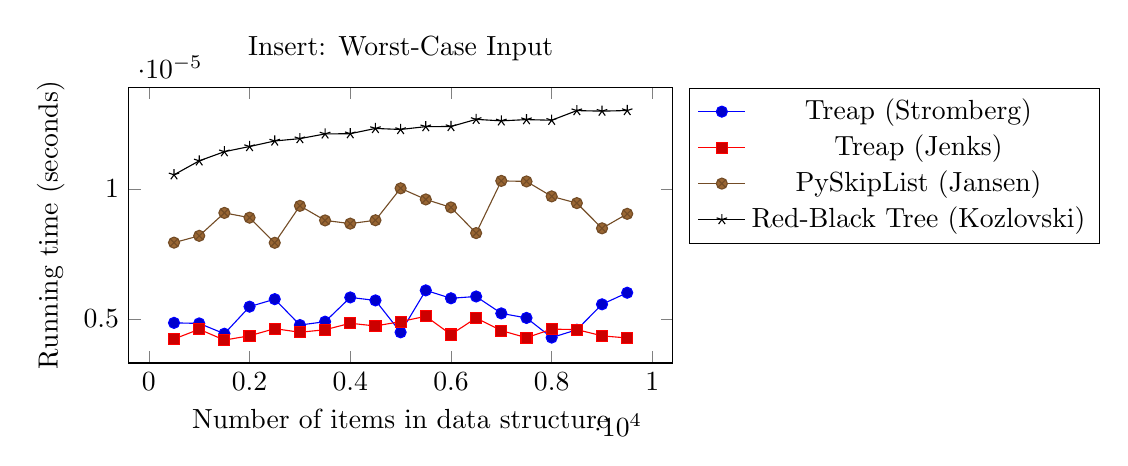
\begin{tikzpicture}
        \begin{axis}[
            xlabel={Number of items in data structure},
            ylabel={Running time (seconds)},
            title={Insert: Worst-Case Input},
            width=0.7\textwidth,
            height=2in,
            legend pos=outer north east
        ]
		\addplot coordinates {
			(500, 4.851934675080827e-06)
			(1000, 4.830852401482844e-06)
			(1500, 4.433300956989683e-06)
			(2000, 5.475367622160832e-06)
			(2500, 5.764495945399517e-06)
			(3000, 4.767605580795475e-06)
			(3500, 4.897110975576879e-06)
			(4000, 5.83075451952908e-06)
			(4500, 5.716307891532324e-06)
			(5000, 4.4875125175991574e-06)
			(5500, 6.101812322611977e-06)
			(6000, 5.797625232482062e-06)
			(6500, 5.866895559911711e-06)
			(7000, 5.216356832562497e-06)
			(7500, 5.0416751372495125e-06)
			(8000, 4.285725041981437e-06)
			(8500, 4.586900378740211e-06)
			(9000, 5.565720223188464e-06)
			(9500, 6.011459721548817e-06)
		};
		\addplot coordinates {
			(500, 4.231513481336435e-06)
			(1000, 4.604970898931526e-06)
			(1500, 4.189348934211523e-06)
			(2000, 4.354995369446613e-06)
			(2500, 4.629064925865123e-06)
			(3000, 4.490524270970297e-06)
			(3500, 4.586900378740211e-06)
			(4000, 4.836875908260652e-06)
			(4500, 4.731464540377317e-06)
			(5000, 4.90012272894802e-06)
			(5500, 5.104921957936881e-06)
			(6000, 4.4031834233138055e-06)
			(6500, 5.041675137213985e-06)
			(7000, 4.553771091693193e-06)
			(7500, 4.2797015352391556e-06)
			(8000, 4.61099440563828e-06)
			(8500, 4.592923885482492e-06)
			(9000, 4.351983616039945e-06)
			(9500, 4.270666275125734e-06)
		};
		\addplot coordinates {
			(500, 7.938981876804974e-06)
			(1000, 8.201004419738923e-06)
			(1500, 9.083448156417263e-06)
			(2000, 8.899731200990858e-06)
			(2500, 7.932958370062693e-06)
			(3000, 9.354505959535686e-06)
			(3500, 8.794319833143049e-06)
			(4000, 8.6708379450684e-06)
			(4500, 8.80034333988533e-06)
			(5000, 1.0029138713818498e-05)
			(5500, 9.60146973564946e-06)
			(6000, 9.294270892148404e-06)
			(6500, 8.30641578758673e-06)
			(7000, 1.0315255283757097e-05)
			(7500, 1.0294173010194641e-05)
			(8000, 9.718928116981829e-06)
			(8500, 9.459917327383493e-06)
			(9000, 8.490132743013135e-06)
			(9500, 9.047307116034632e-06)
		};
		\addplot coordinates {
			(500, 1.0550172046421835e-05)
			(1000, 1.1086264145809821e-05)
			(1500, 1.1438639289806928e-05)
			(2000, 1.1637415012089036e-05)
			(2500, 1.1851249501155791e-05)
			(3000, 1.1941602102218952e-05)
			(3500, 1.2122307304274216e-05)
			(4000, 1.213134256435211e-05)
			(4500, 1.2333130040005359e-05)
			(5000, 1.2293977246216059e-05)
			(5500, 1.2402400367435007e-05)
			(6000, 1.240842387414176e-05)
			(6500, 1.2682493430595799e-05)
			(7000, 1.2625270116650712e-05)
			(7500, 1.2673458170517903e-05)
			(8000, 1.264936414354878e-05)
			(8500, 1.3019809807808257e-05)
			(9000, 1.2998727534210275e-05)
			(9500, 1.3022821561143872e-05)
		};
        \legend{Treap (Stromberg), Treap (Jenks), PySkipList (Jansen), Red-Black Tree (Kozlovski)}
        \end{axis}
    \end{tikzpicture}
    \caption{Average of 100 operations, benchmarked every 500, starting at 500.}
\end{figure}
\begin{figure}[h]
    \centering
    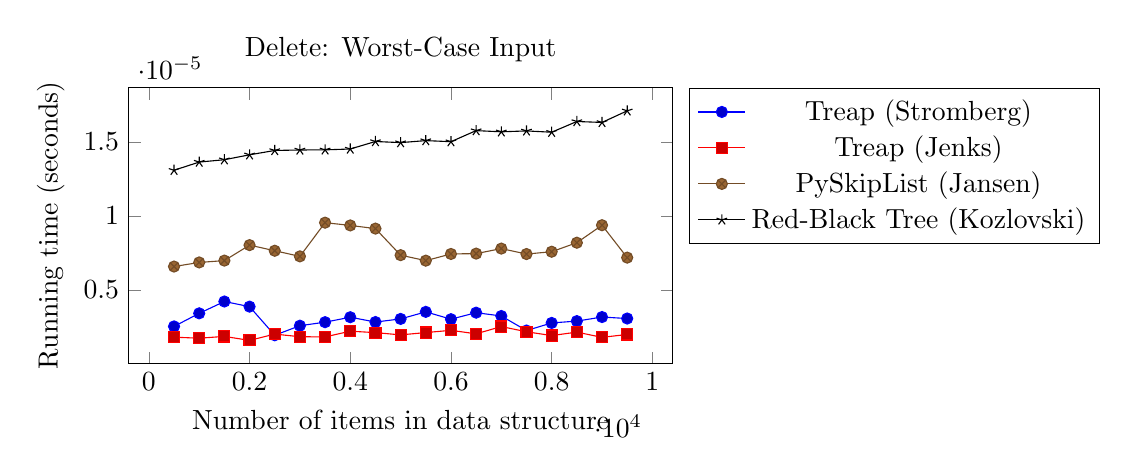
\begin{tikzpicture}
        \begin{axis}[
            xlabel={Number of items in data structure},
            ylabel={Running time (seconds)},
            title={Delete: Worst-Case Input},
            width=0.7\textwidth,
            height=2in,
            legend pos=outer north east
        ]
		\addplot coordinates {
			(9500, 3.0810236949463387e-06)
			(9000, 3.1804115560873923e-06)
			(8500, 2.906341999633355e-06)
			(8000, 2.782860111594232e-06)
			(7500, 2.267850285733175e-06)
			(7000, 3.2496818835170416e-06)
			(6500, 3.475563386103886e-06)
			(6000, 3.035847394414759e-06)
			(5500, 3.5297749467133597e-06)
			(5000, 3.0539179146416017e-06)
			(4500, 2.8430951788749325e-06)
			(4000, 3.168364542673885e-06)
			(3500, 2.8340599187970383e-06)
			(3000, 2.5961314027966864e-06)
			(2500, 1.9516161821542253e-06)
			(2000, 3.882150090745995e-06)
			(1500, 4.228501727965295e-06)
			(1000, 3.430387085572306e-06)
			(500, 2.547943348858439e-06)
		};
		\addplot coordinates {
			(9500, 2.0058277427636993e-06)
			(9000, 1.8100637738882598e-06)
			(8500, 2.1624389178498403e-06)
			(8000, 1.9305339085207154e-06)
			(7500, 2.186532944818964e-06)
			(7000, 2.538908088851599e-06)
			(6500, 2.047992289959666e-06)
			(6000, 2.28290905255335e-06)
			(5500, 2.1323213842094903e-06)
			(5000, 1.975710209052295e-06)
			(4500, 2.1293096308028226e-06)
			(4000, 2.2256857385372085e-06)
			(3500, 1.8401813075996642e-06)
			(3000, 1.8522283210131717e-06)
			(2500, 2.029921769732823e-06)
			(2000, 1.6052645449349256e-06)
			(1500, 1.8733105946466821e-06)
			(1000, 1.7528404598721181e-06)
			(500, 1.8221107873017673e-06)
		};
		\addplot coordinates {
			(9500, 7.1890552882081235e-06)
			(9000, 9.375588233098142e-06)
			(8500, 8.194980912961114e-06)
			(8000, 7.586606732772339e-06)
			(7500, 7.429995557686197e-06)
			(7000, 7.797429468539008e-06)
			(6500, 7.460113091326548e-06)
			(6000, 7.4360190644284786e-06)
			(5500, 6.984256059254789e-06)
			(5000, 7.354701723514267e-06)
			(4500, 9.14669497710463e-06)
			(4000, 9.360529466277967e-06)
			(3500, 9.547258175075513e-06)
			(3000, 7.2733843825290026e-06)
			(2500, 7.652865306866374e-06)
			(2000, 8.032346231132693e-06)
			(1500, 6.987267812590403e-06)
			(1000, 6.86378592455128e-06)
			(500, 6.586704614761629e-06)
		};
		\addplot coordinates {
			(9500, 1.7091700360651885e-05)
			(9000, 1.6308644485150127e-05)
			(8500, 1.637189130576644e-05)
			(8000, 1.5649070497616434e-05)
			(7500, 1.5736411345272927e-05)
			(7000, 1.567617627792117e-05)
			(6500, 1.5757493618835384e-05)
			(6000, 1.50105787836452e-05)
			(5500, 1.5082860864481517e-05)
			(5000, 1.4947331962957832e-05)
			(4500, 1.5022625797129763e-05)
			(4000, 1.4516651231417655e-05)
			(3500, 1.4459427917401513e-05)
			(3000, 1.4450392657394672e-05)
			(2500, 1.4417263370276601e-05)
			(2000, 1.4125123293666774e-05)
			(1500, 1.379383042326765e-05)
			(1000, 1.3634207494703787e-05)
			(500, 1.30830566284601e-05)
		};
        \legend{Treap (Stromberg), Treap (Jenks), PySkipList (Jansen), Red-Black Tree (Kozlovski)}
        \end{axis}
    \end{tikzpicture}
    \caption{Average of 100 operations, benchmarked every 500, starting at 500.}
\end{figure}

\todo{Add any other input sets discussed here.}


- Randomized
- Well-known worst case
- Real-world data sets?
- Randomized sequence of insertions, searches, and deletes
- Much larger data sets

- Use a single ISDBenchmark class to produce 3 standard benchmarks
- Update the project files section to describe/list it
- Update the project files section's description of BenchmarkPlot accordingly

\todo{Finish this section}

\todo{Section: Asymptotic Expectations - talk about expected/average performance. (Talk about it in each subjection.)}
\newpage

\section{Chosen}



\section{Candidates}
% \begin{figure}[h]
    \centering
    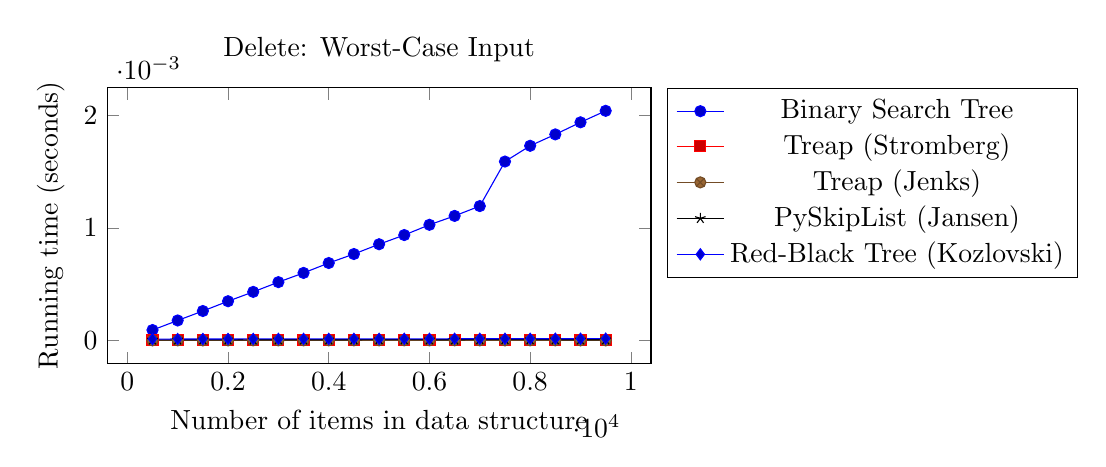
\begin{tikzpicture}
        \begin{axis}[
            xlabel={Number of items in data structure},
            ylabel={Running time (seconds)},
            title={Delete: Worst-Case Input},
            width=0.7\textwidth,
            height=2in,
            legend pos=outer north east
        ]
		\addplot coordinates {
			(9500, 0.0020412429506147765)
			(9000, 0.001939283052110863)
			(8500, 0.0018318899505319487)
			(8000, 0.0017306950373833984)
			(7500, 0.0015906334470270345)
			(7000, 0.0011948499017415592)
			(6500, 0.001107680724025517)
			(6000, 0.001028574010074319)
			(5500, 0.0009375527998012245)
			(5000, 0.000855919224774695)
			(4500, 0.0007689668933011085)
			(4000, 0.0006889506298329274)
			(3500, 0.0006010526078019396)
			(3000, 0.0005191630337391828)
			(2500, 0.00043245766604172787)
			(2000, 0.0003495230135604288)
			(1500, 0.00026249840000602375)
			(1000, 0.00017862106872069462)
			(500, 9.334327211945492e-05)
		};
		\addplot coordinates {
			(9500, 3.6954213819484492e-06)
			(9000, 3.2677524037794115e-06)
			(8500, 2.6443194566994066e-06)
			(8000, 2.3853086670655443e-06)
			(7500, 2.873212712586337e-06)
			(7000, 3.123188242106778e-06)
			(6500, 3.5809747539872206e-06)
			(6000, 3.5267631933422196e-06)
			(5500, 3.7104801487686247e-06)
			(5000, 2.5569786090073875e-06)
			(4500, 3.4454458524280087e-06)
			(4000, 3.4514693591702894e-06)
			(3500, 2.852130439059408e-06)
			(3000, 2.7406955644337925e-06)
			(2500, 3.4605046192481837e-06)
			(2000, 3.243658376810288e-06)
			(1500, 2.466626007979755e-06)
			(1000, 2.8159893986412498e-06)
			(500, 2.788883618336513e-06)
		};
		\addplot coordinates {
			(9500, 1.569123504445713e-06)
			(9000, 1.650440845395451e-06)
			(8500, 1.912463388364927e-06)
			(8000, 1.9726984557166815e-06)
			(7500, 1.6444173386531703e-06)
			(7000, 1.939569168705191e-06)
			(6500, 2.376273406952123e-06)
			(6000, 1.8130755272594001e-06)
			(5500, 2.3943439271789657e-06)
			(5000, 2.0871450837134377e-06)
			(4500, 2.1202743707604554e-06)
			(4000, 2.1684624246276486e-06)
			(3500, 1.9335456619273826e-06)
			(3000, 1.8221107873372944e-06)
			(2500, 2.0178747562482612e-06)
			(2000, 1.710675912747206e-06)
			(1500, 1.5480412309187842e-06)
			(1000, 2.0118512494704534e-06)
			(500, 1.6414055852820297e-06)
		};
		\addplot coordinates {
			(9500, 7.54745393898304e-06)
			(9000, 7.1137614540717205e-06)
			(8500, 7.848629275741814e-06)
			(8000, 8.216063186594624e-06)
			(7500, 8.767214052838313e-06)
			(7000, 8.80034333988533e-06)
			(6500, 6.924020991903035e-06)
			(6000, 7.800441221874622e-06)
			(5500, 8.110651818746817e-06)
			(5000, 8.529285536802433e-06)
			(4500, 7.30350191620488e-06)
			(4000, 7.1679730146811944e-06)
			(3500, 7.27338438256453e-06)
			(3000, 7.7914059617612e-06)
			(2500, 6.3999759059996106e-06)
			(2000, 7.270372629157862e-06)
			(1500, 7.544442185647426e-06)
			(1000, 6.731268776398735e-06)
			(500, 6.580681108019348e-06)
		};
		\addplot coordinates {
			(9500, 1.7085676853909604e-05)
			(9000, 1.643513812652486e-05)
			(8500, 1.6450196893380564e-05)
			(8000, 1.574243485201521e-05)
			(7500, 1.5769540632319946e-05)
			(7000, 1.5778575892433368e-05)
			(6500, 1.5796646412624683e-05)
			(6000, 1.5185260479029238e-05)
			(5500, 1.523043677956082e-05)
			(5000, 1.5046719824134414e-05)
			(4500, 1.5173213465544678e-05)
			(4000, 1.4619050845929848e-05)
			(3500, 1.4576886298804936e-05)
			(3000, 1.4613027339187567e-05)
			(2500, 1.4534721751644497e-05)
			(2000, 1.426065219519046e-05)
			(1500, 1.381792445016572e-05)
			(1000, 1.3579995934165368e-05)
			(500, 1.301077454765931e-05)
		};
        \legend{Binary Search Tree, Treap (Stromberg), Treap (Jenks), PySkipList (Jansen), Red-Black Tree (Kozlovski)}
        \end{axis}
    \end{tikzpicture}
    \caption{Average of 100 operations, benchmarked every 500, starting at 500.}
\end{figure}
% \begin{figure}[h]
    \centering
    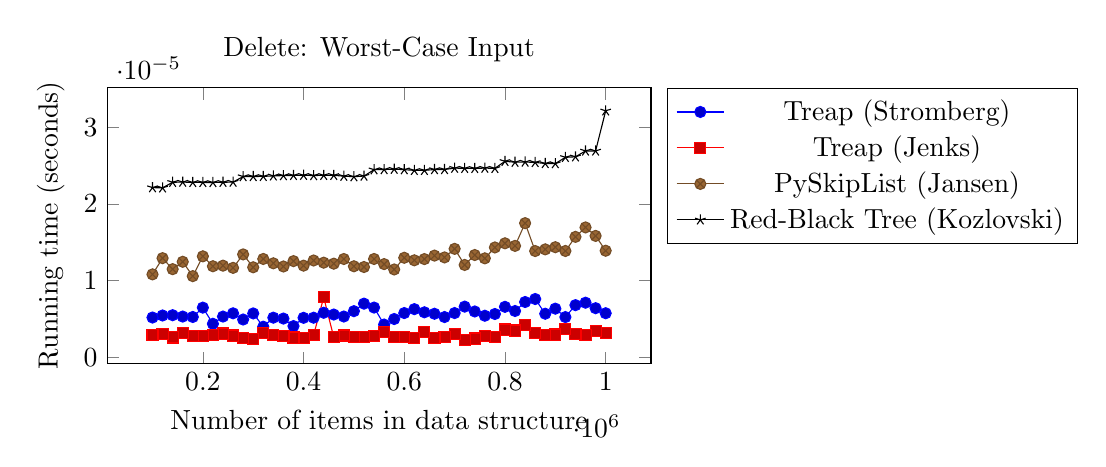
\begin{tikzpicture}
        \begin{axis}[
            xlabel={Number of items in data structure},
            ylabel={Running time (seconds)},
            title={Delete: Worst-Case Input},
            width=0.7\textwidth,
            height=2in,
            legend pos=outer north east
        ]
		\addplot coordinates {
			(1000000, 5.766302997443517e-06)
			(980000, 6.42678051094947e-06)
			(960000, 7.141168409717125e-06)
			(940000, 6.822223728107701e-06)
			(920000, 5.266653113778829e-06)
			(900000, 6.3638348655672416e-06)
			(880000, 5.702453826060605e-06)
			(860000, 7.6212418965013735e-06)
			(840000, 7.230617484736967e-06)
			(820000, 6.05904542477731e-06)
			(800000, 6.600558680247559e-06)
			(780000, 5.667517486998009e-06)
			(760000, 5.439828932409796e-06)
			(740000, 5.997605656077099e-06)
			(720000, 6.627965635900068e-06)
			(700000, 5.789493498383536e-06)
			(680000, 5.271170743839093e-06)
			(660000, 5.698538546681675e-06)
			(640000, 5.888881359496168e-06)
			(620000, 6.300889220185013e-06)
			(600000, 5.79039702438422e-06)
			(580000, 5.013364655567898e-06)
			(560000, 4.2902426720274886e-06)
			(540000, 6.507194325862997e-06)
			(520000, 7.01768652164958e-06)
			(500000, 6.03766197585287e-06)
			(480000, 5.3398387206016195e-06)
			(460000, 5.597343633525043e-06)
			(440000, 5.8283451168108514e-06)
			(420000, 5.18382989616839e-06)
			(400000, 5.169072304667566e-06)
			(380000, 4.0926716511222594e-06)
			(360000, 5.071792670904074e-06)
			(340000, 5.18985340289646e-06)
			(320000, 4.0119566608609605e-06)
			(300000, 5.742811321184149e-06)
			(280000, 4.948913133503652e-06)
			(260000, 5.757267737351413e-06)
			(240000, 5.333514038539988e-06)
			(220000, 4.389931708487893e-06)
			(200000, 6.4993637671051375e-06)
			(180000, 5.279603653249864e-06)
			(160000, 5.33381521387355e-06)
			(140000, 5.512713363899025e-06)
			(120000, 5.474765271472392e-06)
			(100000, 5.206418046427075e-06)
		};
		\addplot coordinates {
			(1000000, 3.177098627389796e-06)
			(980000, 3.4026789546288683e-06)
			(960000, 2.93676070866411e-06)
			(940000, 3.0189815755932157e-06)
			(920000, 3.693011979251537e-06)
			(900000, 2.9900687432729002e-06)
			(880000, 2.8768268166601275e-06)
			(860000, 3.2279972593016735e-06)
			(840000, 4.190252460219312e-06)
			(820000, 3.5108009005142547e-06)
			(800000, 3.634885139263133e-06)
			(780000, 2.7202156415455647e-06)
			(760000, 2.8313493408091974e-06)
			(740000, 2.4618072026072468e-06)
			(720000, 2.226589264608947e-06)
			(700000, 3.062350824080795e-06)
			(680000, 2.7045545240298453e-06)
			(660000, 2.5142117112011418e-06)
			(640000, 3.295460534729955e-06)
			(620000, 2.529270478035528e-06)
			(600000, 2.6569688208297748e-06)
			(580000, 2.6647993795876345e-06)
			(560000, 3.359008530779306e-06)
			(540000, 2.782860111580021e-06)
			(520000, 2.7138909594697224e-06)
			(500000, 2.653053541450845e-06)
			(480000, 2.863273926493548e-06)
			(460000, 2.631067741859283e-06)
			(440000, 7.842605769013744e-06)
			(420000, 2.921701941829724e-06)
			(400000, 2.5861926166896866e-06)
			(380000, 2.597034928811581e-06)
			(360000, 2.85182926369032e-06)
			(340000, 2.9180878377843554e-06)
			(320000, 3.1611363345405154e-06)
			(300000, 2.396753329875878e-06)
			(280000, 2.500056470381651e-06)
			(260000, 2.8608645238108466e-06)
			(240000, 3.121682365431866e-06)
			(220000, 2.9009208436008292e-06)
			(200000, 2.777740130866846e-06)
			(180000, 2.8183988013239513e-06)
			(160000, 3.184326835480533e-06)
			(140000, 2.6145030983428795e-06)
			(120000, 3.047593232594181e-06)
			(100000, 2.8765256413123553e-06)
		};
		\addplot coordinates {
			(1000000, 1.3917011135959e-05)
			(980000, 1.5852062674582612e-05)
			(960000, 1.6957074985128885e-05)
			(940000, 1.572496668248391e-05)
			(920000, 1.3885688900927562e-05)
			(900000, 1.4377809401167951e-05)
			(880000, 1.4095306935303142e-05)
			(860000, 1.387755716683614e-05)
			(840000, 1.7513044656766396e-05)
			(820000, 1.4548876992449778e-05)
			(800000, 1.4885289843618921e-05)
			(780000, 1.4344378938801584e-05)
			(760000, 1.2925541927387486e-05)
			(740000, 1.3357126184956768e-05)
			(720000, 1.2063578113583162e-05)
			(700000, 1.4160963158730055e-05)
			(680000, 1.3045710886729011e-05)
			(660000, 1.3281230000075084e-05)
			(640000, 1.282796111826201e-05)
			(620000, 1.2668940540464747e-05)
			(600000, 1.2999631060210959e-05)
			(580000, 1.1473876804217298e-05)
			(560000, 1.2174410637499023e-05)
			(540000, 1.2841212833080817e-05)
			(520000, 1.1794026187203599e-05)
			(500000, 1.1890101119604424e-05)
			(480000, 1.2836695203048976e-05)
			(460000, 1.2230128074833147e-05)
			(440000, 1.2361139346296569e-05)
			(420000, 1.2645147688857605e-05)
			(400000, 1.1972623161881302e-05)
			(380000, 1.25611197698845e-05)
			(360000, 1.186148946263188e-05)
			(340000, 1.2276509076656339e-05)
			(320000, 1.2844224586444852e-05)
			(300000, 1.175878867280744e-05)
			(280000, 1.343874470117612e-05)
			(260000, 1.1683494838592878e-05)
			(240000, 1.1971117285185073e-05)
			(220000, 1.189522110033181e-05)
			(200000, 1.3187865645676311e-05)
			(180000, 1.060498595768422e-05)
			(160000, 1.2476489500272692e-05)
			(140000, 1.1514234299340842e-05)
			(120000, 1.2949033603632642e-05)
			(100000, 1.0835083914997767e-05)
		};
		\addplot coordinates {
			(1000000, 3.215799658164542e-05)
			(980000, 2.6927785683625417e-05)
			(960000, 2.692507510559494e-05)
			(940000, 2.6163402678946567e-05)
			(920000, 2.6093831176183357e-05)
			(900000, 2.5278549539564212e-05)
			(880000, 2.529210242971658e-05)
			(860000, 2.543184778599539e-05)
			(840000, 2.5482144067240143e-05)
			(820000, 2.545654416360321e-05)
			(800000, 2.5577014298306723e-05)
			(780000, 2.4658429521196012e-05)
			(760000, 2.4688245879559644e-05)
			(740000, 2.465150248846726e-05)
			(720000, 2.466415185259052e-05)
			(700000, 2.4684631775500065e-05)
			(680000, 2.4511154781521326e-05)
			(660000, 2.4504227748792574e-05)
			(640000, 2.4396105802907188e-05)
			(620000, 2.439339522484829e-05)
			(600000, 2.44897713326111e-05)
			(580000, 2.4548500523280835e-05)
			(560000, 2.450332422279189e-05)
			(540000, 2.4478929020517625e-05)
			(520000, 2.3653407422443705e-05)
			(500000, 2.3569680678861004e-05)
			(480000, 2.363774630495641e-05)
			(460000, 2.374948235487295e-05)
			(440000, 2.37500847055685e-05)
			(420000, 2.3720268347233286e-05)
			(400000, 2.375731291363081e-05)
			(380000, 2.3736230640054145e-05)
			(360000, 2.3712738963808987e-05)
			(340000, 2.3676296748050162e-05)
			(320000, 2.3609435823289005e-05)
			(300000, 2.3595280582469514e-05)
			(280000, 2.358654649771097e-05)
			(260000, 2.28655327415197e-05)
			(240000, 2.284354694194235e-05)
			(220000, 2.2815537635608506e-05)
			(200000, 2.282216349303212e-05)
			(180000, 2.2822765843699244e-05)
			(160000, 2.2867038618215928e-05)
			(140000, 2.2844149292637894e-05)
			(120000, 2.2114100276326097e-05)
			(100000, 2.2145121336023977e-05)
		};
        \legend{Treap (Stromberg), Treap (Jenks), PySkipList (Jansen), Red-Black Tree (Kozlovski)}
        \end{axis}
    \end{tikzpicture}
    \caption{Average of 1000 operations, benchmarked every 20000, starting at 100000.}
\end{figure}
% \begin{figure}[h]
    \centering
    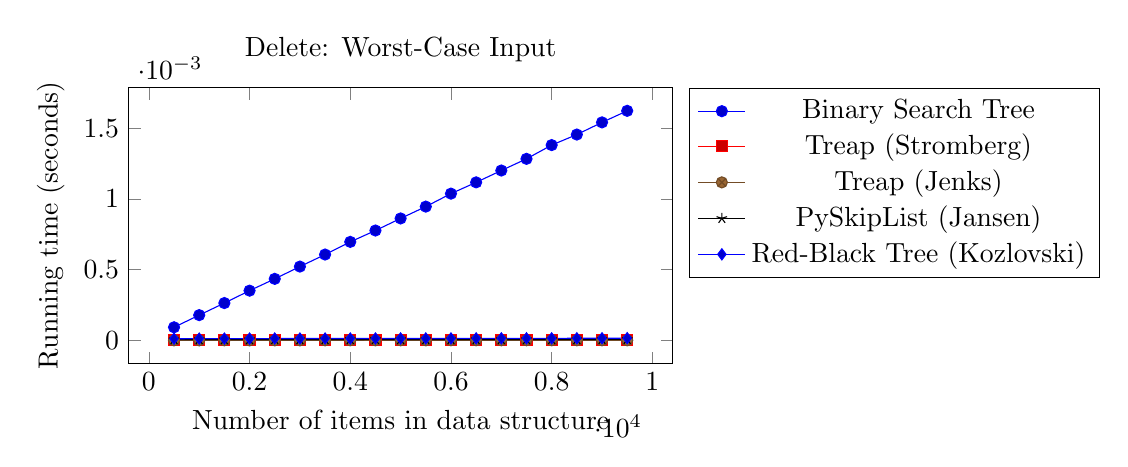
\begin{tikzpicture}
        \begin{axis}[
            xlabel={Number of items in data structure},
            ylabel={Running time (seconds)},
            title={Delete: Worst-Case Input},
            width=0.7\textwidth,
            height=2in,
            legend pos=outer north east
        ]
		\addplot coordinates {
			(9500, 0.0016222177045921882)
			(9000, 0.0015406925526868776)
			(8500, 0.0014547642173582177)
			(8000, 0.0013802986153464048)
			(7500, 0.0012832930511320485)
			(7000, 0.0012008463026962346)
			(6500, 0.0011172370174606528)
			(6000, 0.001037600234916809)
			(5500, 0.0009460098032571551)
			(5000, 0.0008624517178288471)
			(4500, 0.0007771799447343141)
			(4000, 0.0006969859878174844)
			(3500, 0.0006075911243627985)
			(3000, 0.0005225723385512282)
			(2500, 0.00043581577104646386)
			(2000, 0.00035254982569476567)
			(1500, 0.0002649740612741169)
			(1000, 0.0001798227583142875)
			(500, 9.393959928623019e-05)
		};
		\addplot coordinates {
			(9500, 4.168266660684594e-06)
			(9000, 4.3790893963091545e-06)
			(8500, 4.192360687582664e-06)
			(8000, 3.764691709449153e-06)
			(7500, 4.171278414020208e-06)
			(7000, 3.936361651355469e-06)
			(6500, 3.2105290897277427e-06)
			(6000, 3.1412587622980938e-06)
			(5500, 2.972600573727391e-06)
			(5000, 3.4635163726193243e-06)
			(4500, 3.352081498064763e-06)
			(4000, 2.6473312100705472e-06)
			(3500, 2.5901078960544056e-06)
			(3000, 2.7135897841645827e-06)
			(2500, 2.538908088851599e-06)
			(2000, 3.361116758142657e-06)
			(1500, 3.1382470089624803e-06)
			(1000, 2.8973067395554607e-06)
			(500, 2.7256367975780904e-06)
		};
		\addplot coordinates {
			(9500, 2.041968783217385e-06)
			(9000, 2.376273406952123e-06)
			(8500, 2.20761521838142e-06)
			(8000, 2.246768012170719e-06)
			(7500, 2.219662231865982e-06)
			(7000, 2.047992289959666e-06)
			(6500, 2.4786730214998443e-06)
			(6000, 2.5298728287026505e-06)
			(5500, 1.8793341013889631e-06)
			(5000, 1.927522155185102e-06)
			(4500, 1.8371695541929967e-06)
			(4000, 1.936557415262996e-06)
			(3500, 2.099192097162472e-06)
			(3000, 1.5450294775121165e-06)
			(2500, 1.6986288992626442e-06)
			(2000, 1.4366063563642228e-06)
			(1500, 2.111239110647034e-06)
			(1000, 1.5751470112235211e-06)
			(500, 1.7648874733566799e-06)
		};
		\addplot coordinates {
			(9500, 8.941895748151296e-06)
			(9000, 8.210039679852343e-06)
			(8500, 7.249290355630933e-06)
			(8000, 7.613712513077075e-06)
			(7500, 7.556489199060934e-06)
			(7000, 7.74321790785848e-06)
			(6500, 7.532395172162865e-06)
			(6000, 6.779456830230402e-06)
			(5500, 7.695029853991287e-06)
			(5000, 7.571547965952164e-06)
			(4500, 8.219074939930238e-06)
			(4000, 7.881758562788832e-06)
			(3500, 7.008350086223913e-06)
			(3000, 6.707174749465139e-06)
			(2500, 8.047404998023922e-06)
			(2000, 7.170984768052335e-06)
			(1500, 6.571645847941454e-06)
			(1000, 7.059549893497774e-06)
			(500, 6.761386310074613e-06)
		};
		\addplot coordinates {
			(9500, 1.7112782634285394e-05)
			(9000, 1.6335750265383808e-05)
			(8500, 1.639899708614223e-05)
			(8000, 1.5730387838530646e-05)
			(7500, 1.5679188031256784e-05)
			(7000, 1.5673164524514506e-05)
			(6500, 1.570930556496819e-05)
			(6000, 1.5079849111145905e-05)
			(5500, 1.5073825604474678e-05)
			(5000, 1.5031661057278711e-05)
			(4500, 1.5034672810614324e-05)
			(4000, 1.4570862792027128e-05)
			(3500, 1.4507615971268705e-05)
			(3000, 1.4468463177550461e-05)
			(2500, 1.4417263370276601e-05)
			(2000, 1.4137170307151337e-05)
			(1500, 1.3845030230470456e-05)
			(1000, 1.3790818669860983e-05)
			(500, 1.305896260156203e-05)
		};
        \legend{Binary Search Tree, Treap (Stromberg), Treap (Jenks), PySkipList (Jansen), Red-Black Tree (Kozlovski)}
        \end{axis}
    \end{tikzpicture}
    \caption{Average of 100 operations, benchmarked every 500, starting at 500.}
\end{figure}
% \input{plots/worstCase_insert4.tex}
% \input{plots/worstCase_insert5.tex}
% \input{plots/worstCase_insert6.tex}
% \input{plots/worstCase_insert7.tex}
% \input{plots/worstCase_insert8.tex}
% \input{plots/worstCase_insert9.tex}
% \input{plots/worstCase_insert10.tex}

\end{document}
